\chapter{Neexpandující impulzní gravitační vlny}
\label{chap:kap02}
V této kapitole se budeme věnovat neexpandujícím impulzním gravitačním vlnám propagujícím se na pozadí Minkowského a (anti--)de Sitterova
prostoročasu. Popíšeme matematickou konstrukci prostoročasů, která vede k takzvaným refrakčním rovnícím pro geodetiky a které dále využijeme k vizualizaci účinku
impulzních řešení a k interpretaci jejich působení na různé konfigurace testovacích částic.


\section{Konstrukce prostoročasu}
Nejprve intuitivně popíšeme konstrukci prostoročasů s neexpandujícími impulzními gravitačními vlnami
pomocí Penroseovy geometrické metody \cite{Penrose:1972xrn} označované jako "cut and paste". Následně zavedeme souřadnice, ve
kterých je metrika spojitá, a dále se budeme věnovat přirozenému distribučnímu popisu prostoročasů s impulzními gravitačními
vlnami. Tento přístup byl detailně popsán a prozkoumán v \cite{Podolsky:2014ysa}.

\subsection{"Cut and paste"\ metoda}
\label{sec:cut_and_paste_konstrukce1}
Geometrická metoda konstrukce "cut and paste"\ impulzních gravitačních vln v~Minkowského prostoročase \eqref{eq:minkowski} se zakládá na rozdělení celého prostoročasu podél rovinné
světelné nadplochy $\mathcal{N}$, kde bude výsledná implulzní vlna lokalizována na dvě části $\mathcal{M}^+$ a $\mathcal{M}^-$. Opětovným spojením těchto částí a ztotožněním bodů na hranici
řezu $\mathcal{N}$ se specifickým posunutím dostaneme prostoročas s impulzní gravitační vlnou.

\begin{figure}[ht]\centering
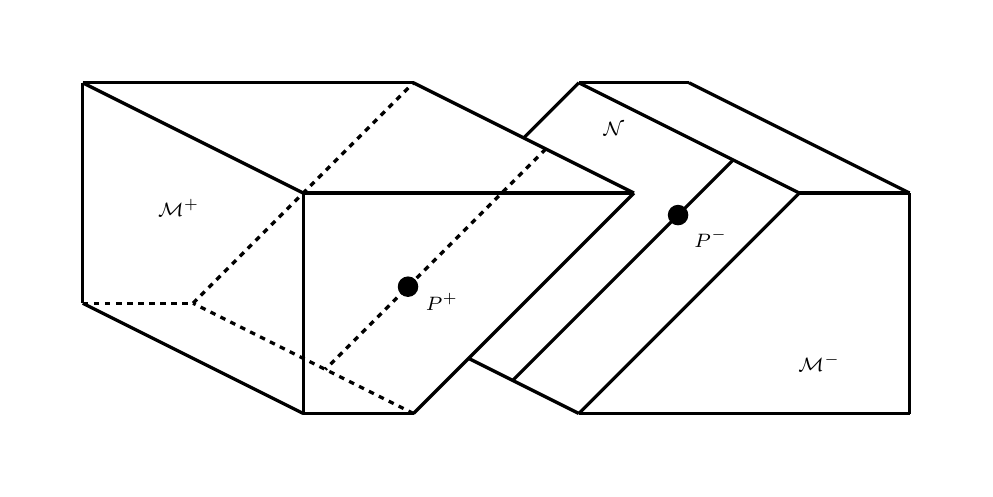
\begin{tikzpicture}[scale=1.4]
\clip(-2.5,-0.5) rectangle (6.,3.5);
\draw [line width=1.2pt] (-2.,1.)-- (0.,0.);
\draw [line width=1.2pt] (-2.,3.)-- (-2.,1.);
\draw [line width=1.2pt] (0.,0.)-- (0.,2.);
\draw [line width=1.2pt] (0.,2.)-- (-2.,3.);
\draw [line width=1.2pt] (-2.,3.)-- (1.,3.);
\draw [line width=1.2pt] (0.,2.)-- (3.,2.);
\draw [line width=1.2pt] (1.,3.)-- (3.,2.);
\draw [line width=1.2pt] (0.,0.)-- (1.,0.);
\draw [line width=1.2pt] (1.,0.)-- (3.,2.);
\draw [line width=1.2pt,dash pattern=on 2pt off 2pt] (1.,0.)-- (-1.,1.);
\draw [line width=1.2pt,dash pattern=on 2pt off 2pt] (-2.,1.)-- (-1.,1.);
\draw [line width=1.2pt,dash pattern=on 2pt off 2pt] (-1.,1.)-- (1.,3.);
\draw [line width=1.2pt] (2.5,0.)-- (4.5,2.);
\draw [line width=1.2pt] (2.5,0.)-- (5.5,0.);
\draw [line width=1.2pt] (5.5,0.)-- (5.5,2.);
\draw [line width=1.2pt] (4.5,2.)-- (5.5,2.);
\draw [line width=1.2pt] (4.5,2.)-- (2.5,3.);
\draw [line width=1.2pt] (5.5,2.)-- (3.5,3.);
\draw [line width=1.2pt] (2.5,3.)-- (3.5,3.);
\draw [line width=1.2pt] (2.,2.5)-- (2.5,3.);
\draw [line width=1.2pt] (2.5,0.)-- (1.5,0.5);
\draw [line width=1.2pt] (1.9,0.3)-- (3.9,2.3);
\draw [line width=1.2pt,dash pattern=on 2pt off 2pt] (2.2,2.4)-- (0.2,0.4);
\begin{scriptsize}
\draw[color=black] (-1.1302677200189184,1.864045432930641) node {$\mathcal{M}^+$};
\draw[color=black] (2.8186222701156605,2.585603404549911) node {$\mathcal{N}$};
\draw[color=black] (4.6815537604781525,0.46028719723496975) node {$\mathcal{M}^-$};
\draw [fill=black] (0.9503176308657735,1.1503176308657732) circle (2.5pt);
\draw[color=black] (1.2574332042485015,1.0112951028351398) node {$P^+$};
\draw [fill=black] (3.4,1.8) circle (2.5pt);
\draw[color=black] (3.6976110719064135,1.5885414801305562) node {$P^-$};
\end{scriptsize}
\end{tikzpicture}
\caption{Princip geometrické konstrukce neexpandující impulzní gravitační vlny pomocí metody "cut and paste", 
podél nadplochy $\mathcal{N}$ dojde k rozdělení prostoročasu na dvě části $\mathcal{M}^+$ a $\mathcal{M}^-$ 
a opětovnému ztotožnění bodů na hranici obou částí se specifickým posunem.}
\label{obr01:geomkonstrukt}
\end{figure}

Pro světelnou nadplochu $\mathcal{N}$ danou podmínkou $\mathcal{U}=0$ v adaptovaných souřadnicích pak tato konstrukce odpovídá Penroseovým 
napojovacím (lepícím) podmínkám

\begin{equation}
    \label{eq:lepici_podminky}
\left[\eta, \bar{\eta}, \mathcal{V}, \mathcal{U}=0_- \right]_{\mathcal{M}^-} \equiv 
\left[\eta, \bar{\eta}, \mathcal{V}-H\left(\eta, \bar{\eta}\right), \mathcal{U}=0_+  \right]_{\mathcal{M}^+},
\end{equation}
kde $H(\eta, \bar{\eta})$ je holomorfní funkcí souřadnic příčného prostoru. Penrose \cite{Penrose:1972xrn} ukázal, že impulzní gravitační vlny
jsou v tenzoru křivosti reprezentovány členy proporciálními Diracově delta distribuci $\delta(\mathcal{U})$.
V Minkowského pozadí je nadplocha $\mathcal{U}=0$ rovina a řešení spadá do rodiny takzvancýh impulzních \emph{pp}-vln, tedy
rovnoběžně se propagujících rovinných vln (viz například \cite{griffiths_podolsky_2009}). Obecně na pozadích konstantní křivosti platí stejné napojovací podmínky
\eqref{eq:lepici_podminky},viz \cite{Podolsky:2014ysa}, a nadplocha $\mathcal{U}=0$ +dstavuje plochu konstantní Gaussovské křivosti 
$K=\frac{1}{3}\Lambda$, která je popsána metrikou $d\sigma^2=2(1+\frac{1}{6}\Lambda \eta \bar{\eta})^{-2} 
d\eta~d\bar{\eta}$. V případě $\Lambda \neq 0$ se tedy jedná buďto o sféru
($\Lambda > 0$), nebo o hyperbolickou plochu ($\Lambda < 0$). Popis těchto nadploch konstatní křivostsi v (A)dS prostoročasech a
jejich geometrické vlastnosti jsou shrnuty v \cite{Podolsky:1997ri}, kde je také ukázáno,
že se jedná o neexpandující nadplochy.

\begin{figure}[H]
    \centering
    \begin{tikzpicture}
         \node[inner sep=0pt, anchor=south west] (ds) at (0,0)
        {\adjincludegraphics[trim={{.2\width} {.18\height} {.2\width} {.25\height}}, width=.8\textwidth, clip]{../img/kap02/CutAndPaste_only_past_gen.pdf}};
        \node[text width=5cm, rotate=45, anchor=north] at (7.6,8.6) {\tiny\textcolor{gray}{$\matu = \pm \infty$}};
        \node[text width=5cm, rotate=45, anchor=north] at (5.6,7.2) {\tiny$\matu = 0$};
        \filldraw[white] (0.05,5.4) circle (8pt);
        \node[text width=14pt] at (0.05,5.4) {\normalsize{$Z_0$}};
        \filldraw[white] (4.52,0.5) circle (9pt);
        \node[text width=14pt] at (4.52,0.5) {\normalsize{$Z_1$}};
        \filldraw[white] (10.7,2.2) circle (9pt);
        \node[text width=14pt] at (10.7,2.2) {\normalsize{$Z_4$}};
    \end{tikzpicture}
    \caption{Nulové geodetiky procházející impulzem nacházejícím se v $\matu=0$ (černá čára) v AdS prostoročase jsou podle "cut and paste"\ konstrukce posunuty
    v~souřadnici $\matv$ a dochází k refrakci. Ve spodní polovině jsou vykresleny nulové generátory anti--de Sitterova hyperboloidu.}
\end{figure}

\subsection{Spojitý tvar metriky}
Metoda "cut and paste"\ nám dává identifikaci bodů prostoročasu na obou stranách impulzní vlny, a tedy část\footnote{Jedná se pouze o podmínky napojení poloh, napojení rychlostí
je potřeba diskutovat detailněji, viz \cite{Podolsky:2014ysa}.} napojovacích podmínek
pro geodetiky, nic ale neříká o podobě metriky kompletního prostoročasu s impulzní vlnou. Potřebujeme tedy najít vhodný
souřadnicový systém, ve kterém bude metrika spojitá přes rozhraní $\mathcal{U}=0$. Toho dosáhneme postupem použitým např. v
\cite{Podolsky:2014ysa}, kde z metriky prostoročasu pozadí \eqref{eq:konfmetric}, tedy
\begin{equation}
    \label{eq:null_background_metric}
    \mathrm{d}s_0^2 = \frac{2~\mathrm{d}\eta~\mathrm{d}\bar{\eta}-2~\mathrm{d}\mathcal{U}~\mathrm{d}\mathcal{V}}
    {\left[1+\frac{1}{6}\Lambda \left(\eta \bar{\eta}
    -\mathcal{U}\mathcal{V}\right)\right]^2},
\end{equation}
souřadnicovou transformací
\begin{equation}
    \label{eq:nonexp_cont_transform}
    \mathcal{U}=U,~~~~ \mathcal{V}=V+H+UH_{,Z}H_{,\bar{Z}},~~~~ \eta=Z+UH_{,\bar{Z}},
\end{equation}
kde uvažujeme libovolnou reálnou funkci $H(Z, \bar{Z})$, obdržíme metriku
\begin{equation}
    \label{eq:nonexp_cont_nokink_metric}
    \mathrm{d} s^{2}=\frac{2\left|\mathrm{d} Z-U\left(H_{, Z \bar{Z}} 
    \mathrm{d} Z+H_{, \bar{Z} \bar{Z}} \mathrm{d} \bar{Z}\right)\right|^{2}-2 \mathrm{d} U 
    \mathrm{d} V}{\left[1+\frac{1}{6} \Lambda(Z \bar{Z}-U V-U G)\right]^{2}},
\end{equation}
kde $G(Z, \bar{Z}) \equiv H - Z H_{,Z}-\bar{Z}H_{,\bar{Z}}$. Metriku \eqref{eq:nonexp_cont_nokink_metric} pak 
uvažujeme pouze pro $U>0$, zatímco na $U<0$ provedeme ztotožnení souřadnic
\begin{equation}
    \label{eq:transformation_just_rename}
    \begin{split}
        &\mathcal{U} = U \\
        &\mathcal{V} = V \\
        &\eta = Z
    \end{split}
\end{equation}
a uvažujeme metriku vzniklou právě touto transformací.
Definováním takzvané kink funkce jako
\begin{equation}
    \label{eq:kink_function}
    U_+ \equiv U_+(U) = \begin{cases}
        0 & \text{pro } U \leq 0 \\
        U & \text{pro } U \geq 0
    \end{cases}
\end{equation}
můžeme výslednou metriku zapsat jako
\begin{equation}
    \label{eq:nonexp_continuous_metric}
    \mathrm{d} s^{2}=\frac{2\left|\mathrm{d} Z+U_+\left(H_{, Z \bar{Z}} 
    \mathrm{d} Z+H_{, \bar{Z} \bar{Z}} \mathrm{d} \bar{Z}\right)\right|^{2}-2 \mathrm{d} U 
    \mathrm{d} V}{\left[1+\frac{1}{6} \Lambda(Z \bar{Z}-U V-U_+ G)\right]^{2}}.
\end{equation}
Transformace \eqref{eq:nonexp_cont_transform} a \eqref{eq:transformation_just_rename} spojující separátně pro $\mathcal{U}>0$ a $\mathcal{U}<0$ metriku \eqref{eq:null_background_metric}
s metrikou \eqref{eq:nonexp_continuous_metric} lze pomocí Heavisideovy skokové funkce $\Theta(U)$ přepsat do tvaru 
\begin{equation}
    \label{eq:nonexp_cont_full_transform}
    \mathcal{U}=U,~~~~ \mathcal{V}=V+\Theta(U) H + U_+ H_{,Z}H_{,\bar{Z}},~~~~ \eta=Z+ U_+ H_{,\bar{Z}}.
\end{equation}
Stále je ale nutné provádět transformaci separátně pro $\mathcal{U}>0$ a $\mathcal{U}<0$, Heavisideova funkce
má při transformaci metriky \eqref{eq:null_background_metric} pro všechna $\matu$ za následek vznik členů proporcionálních delta funkci -- formálně tak generuje impulzní tvar metriky. Je také nutné podotknout,
že toto vyjádření je pak ve smyslu distribucí.
Tato transformace spojuje distribuční vyjádření metriky \eqref{eq:nonexp_distr_metric_omega}, které bude zavedeno dále,
se spojitým tvarem metriky \eqref{eq:nonexp_continuous_metric}, ve kterém se distribuční členy metriky a členy vzniké transformací kompenzují.
Transformace \eqref{eq:nonexp_cont_full_transform} zároveň obsahuje Penroseovy spojovací podmínky \eqref{eq:lepici_podminky} v $U=0$, kde
vzniká nespojitost v souřadnici $\mathcal{V}$. Tato metoda konstrukce, ve smyslu distribucí, tedy představuje explicitní realizaci "cut and paste"\ přístupu.


\subsection{Distribuční tvar metriky}
Dalším způsobem konstrukce impulzní gravitační vlny je přechod od příslušných rodin takzvaných "sandwichových"\
gravtiačních vln s hladkým profilem vlnoplochy k limitnímu distribučnímu vyjádření impulzní vlny. Pro případ neexpandujících vln propagujících se
na $\mathbb{E}^{1,3}$ byl tento limitní přechod uvažován např. v \cite{Penrose1968TwistorQuant}, \cite{Podolsky_1998}, \cite{Podolsky_1998_nonexpanding}.
Výsledná metrika nabývá tvaru
\begin{equation}
    \rmd s^2 = 2~ \rmd \xi \rmd \bar{\xi} - 2 \rmd u \rmd v + H(\xi, \bar{\xi}) \delta\left( u\right) \rmd u^2,
\end{equation}

přičemž $\delta(\matu)$ nahrazuje obecný sandwichový profil vlny.
Distribuční tvar metriky také dostaneme dosazením invezní transformace k \eqref{eq:nonexp_cont_full_transform} do spojité metriky 
\eqref{eq:nonexp_continuous_metric}. Vzhledem k nespojitosti v transformaci toto dosazení nemůže být provedeno
v rámci klasické teorie distribucí, kde nelze konzistentně definovat násobení dvou distribucí. S využitím regularizačních metod teorie
nelineárních zobecněných funkcí, které zakládají na Colombeaových algebrách, je ale možné odvodit pravidla pro násobení
jisté třídy distribucí, která dostačují pro toto odvození. Přehled teorie zobecněných distribucí lze nalézt například v \cite{Steinbauer_book}.
Konkrétně potřebujeme mít zavedené násobení distribucí
\begin{equation}
        \Theta^2 = \Theta, ~~~~ \Theta U_{+} = U_{+}.
\end{equation}
Kromě pravidel pro násobení ještě využijeme identity z klasické teorie distribucí
\begin{equation}
    \Theta' = \delta, ~~~~ U_{+}' = \Theta.
\end{equation}
Takto dostáváme pro libovolnou hodnotu $\Lambda$ metriku ve tvaru
\begin{equation} \label{eq:nonexp_distr_metric_omega}
\mathrm{d}s^2=\frac{2\mathrm{d}\eta~\mathrm{d}\bar{\eta} - 2 \mathrm{d}\mathcal{U}~\mathrm{d}\mathcal{V} + 2H(\eta, \bar{\eta}) \delta(\mathcal{U}) 
~\mathrm{d}\mathcal{U}^2}{\left[1+\frac{1}{6}\Lambda(\eta \bar{\eta}-\mathcal{U}\mathcal{V})\right]^2}.
\end{equation}

V případě nenulové kosmologické konstanty můžeme také využít vnoření do $\mathbb{E}^{1,4}$, případně $\mathbb{E}^{2,4}$ (podle znaménka kosmologické
konstanty, jak je popsáno v kapitole\autoref{chap:kap01}) s dodatečným neexpandujícím impulzem
\begin{equation}
    \label{eq:5DDistributionalWaveMetric}
    \rmd s^2 = \rmd Z_2^2 + \rmd Z_3^2 + \epsilon \rmd Z_4^2 - 2 \rmd \tilde{U} \rmd \tilde{V} + \mathcal{H}(Z_2, Z_3, Z_4) \delta(\tilde{U}) \rmd \tilde{U}^2,
\end{equation}
kde $\epsilon = \text{sign} (\Lambda)$, $\tilde{U} = \tfrac{1}{\sqrt{2}}(Z_0 - Z_1)$, $\tilde{V}= \tfrac{1}{\sqrt{2}}(Z_0 + Z_1)$.
S podmínkou analogickou k \eqref{eq:dS_hyperboloid} a \eqref{eq:AdS_hyperboloid},
\begin{equation}
    Z_2^2 + Z_3^2 + \epsilon Z_4^2 - 2 \tilde{U} \tilde{V} = \epsilon a^2,
\end{equation}
dostáváme reprezentaci impulzních vln propagujících se na (A)dS prostoročasu s impulzem na $\tilde{U}=0$. 
Funkce $H$ a $\mathcal{H}$ v metrikách \eqref{eq:nonexp_distr_metric_omega} a \eqref{eq:5DDistributionalWaveMetric} jsou svázány vztahem
\begin{equation}
    \mathcal{H} = \frac{2H}{1+\frac{1}{6}\Lambda \eta \bar{\eta}}.
\end{equation}

impulzní plocha má v těchto souřadnicích tvar
$Z_2^2 + Z_3^2 + \epsilon Z_4^2 = \epsilon a^2,$
a odpovídá tedy, jak již bylo zmíněno, 2-sféře pro $\epsilon=1$ a 2-hyperboloidu pro $\epsilon=-1$.

\section{\texorpdfstring{$\mathcal{C}^1$}{C1}-matching a refrakční rovnice}
Dále budeme explicitně modelovat geodetiky na prostoročasech s neexpandujícími impulzními vlnami v souřadnicích
\eqref{eq:nonexp_distr_metric_omega}. V těchto souřadnicích není řešení rovnice geodetiky dobře definované v
klasické teorii distribucí. Pro neexpandující impulzní vlny na Minkowského prostoročasu byla rovnice geodetiky
a její řešení zkoumána v rámci teorie zobecněných funkcí ve smyslu Colombeaových algeber v článích \cite{Steinbauer_1998} a \cite{Kunzinger_1999},
přičemž byla ukázána existence a jednoznačnost řešení v prostoru těchto funkcí a bylo ověřeno, že geodetiky na $\mathcal{M}^-$ a $\mathcal{M}^+$ odpovídají
geodetikám na Minkowského pozadí se skokem v souřadnici $\matv$ při přechodu přes nadplochu $\matu=0$. V prostoročasech s
nenulovou kosmologickou konstantou lze využít přístup vnoření do pětidimenzionálního Minkowského prostoru, kde se v rovnici
geodetiky nachází pouze výrazy jednoznačně definované v klasické teorii distribucí. Řešení rovnice geodetiky
pro (anti--)de Sitterův prostoročas s impulzními neexpandujícími vlnami byly tímto způsobem odvozeny v \cite{Podolsk__2001}.
V článku \cite{Podolsky:2014ysa} byla odvoena rovnice geodetiky ve spojitých souřadnicích \eqref{eq:nonexp_continuous_metric}.
Odvozený tvar je v tomto případě analyzován ve smyslu Filippovových řešení (diferenciálních inkluzí) \cite{filippov1988differential}, což je zobecnění teorie obyčejných diferenciálních rovnic.
V článku je ukázána existence a jednoznačnost takových řešení, dále autoři využívají metodou $\mathcal{C}^1$-matchingu,
kde při splnění lokální lipschitzovskosti metriky lze řešení ve smyslu Filippovova přiřadit řešením rovnice geodetiky na jednotlivých částech prostoročasu
("před "a "za" impulzem), bez nutné znalosti detailů teorie za Filippovovými řešeními. Prakticky pak pouze přecházíme od
spojitého $C^1$ řešení k souřadnicím explicitně vyjadřujícím impulzní povahu vlny.

Výsledkem $\mathcal{C}^1$-matchingu je sada refrakčních rovnic, které udávají jak skok v~souřadnici $\matv$,
tak i změnu v rychlostech před a za impulzem. Geodetiku procházející impulzní plochou ve spojitých souřadnicích tedy
ztotožníme transformací \eqref{eq:nonexp_cont_full_transform} (a její derivací), v oblastech $U > 0$ a $U < 0$ separátně, s geodetikami v souřadnicích prostoročasu na pozadí.
Pro polohy dostáváme limitou $U \to 0^+$ a $U \to 0^-$ rovnice
\begin{equation}
    \label{eq:refraction_nonexpanding_positions}
    \begin{split}
        \matu^{+}_{\mathrm{i}} &= \matu^{-}_{\mathrm{i}} = 0,\\
        \matv^{+}_{\mathrm{i}} &= \matv^{-}_{\mathrm{i}} + H_{\mathrm{i}},\\
        \eta^{+}_{\mathrm{i}} &= \eta^{-}_{\mathrm{i}},
    \end{split}
\end{equation}
což přesně odpovídá Penroseovým spojovacím podmínkám \eqref{eq:lepici_podminky} - geodetika je spojitá v $\matu$ a $\eta$ a dochází ke skoku ve $\matv$.
Pro rychlosti obdržíme stejnou limitou rovnice
\begin{equation}
    \label{eq:refraction_nonexpanding_velocities}
    \begin{split}
        &\dot{\mathcal{U}}^{+}_{\mathrm{i}} = \dot{\mathcal{U}}^{-}_{\mathrm{i}},\\
        &\dot{\mathcal{V}}^{+}_{\mathrm{i}} = \dot{\mathcal{V}}_{\mathrm{i}}^{-} + H_{\mathrm{i}, Z}
        \dot{\eta}^{-}_{\mathrm{i}} + H_{\mathrm{i}, \bar{Z}} \dot{\overline{\eta}}^{-}_{\mathrm{i}} + 
        H_{\mathrm{i}, Z} H_{\mathrm{i}, \bar{Z}} \dot{\mathcal{U}}_{\mathrm{i}}^{-},\\
        &\dot{\eta}_{\mathrm{i}}^{+} =\dot{\eta}_{\mathrm{i}}^{-}+H_{\mathrm{i}, \bar{Z}}
        \dot{\mathcal{U}}_{\mathrm{i}}^{-}.
    \end{split}
\end{equation}
Index $\rmi$ zde znamená hodnotu na impulzní nadploše $\matu = 0$, složky označené znakem + jsou za impulzem ($\matu > 0$),
složky označené znakem - jsou před impulzem ($\matu <0$).

Všimněme si, že při přechodu přes impulzní plochu platí $\eta_{\mathrm{i}} = Z_{\mathrm{i}}$, a tedy $ H_{\mathrm{i},Z} = \frac{\partial}{\partial \eta} H(\eta, \bar{\eta})\vert_{\matu = 0}$.

Bližším pohledem na refrakční rovnice také vidíme, že zachovávají kauzální charakter. Složka rychlosti $\dot \matu$ se
nemění, ve složkách $\dot \matv$ a $\dot \eta$ dojde k refrakci tak, že nedochází ke změně normy čtyřrychlosti.

Dále uvedeme refrakční rovnice v reálných polárních prostorových souřadnicích, které vychází z transformace spojitých souřadnic
\begin{equation}
    \begin{split}
        \rho &= \sqrt{2} \left|Z + U_{+} H_{,\bar{Z}}\right|, \\
        \varphi &= \frac{1}{2i} \log \frac{Z + U_+ H_{,\bar{Z}}}{\bar{Z} + U_+ H_{,Z}}
    \end{split}
\end{equation}
Limitou $U \to 0^+$ a $U \to 0^-$ dostáváme
\begin{equation}
    \begin{split}
        \matv^{+}_{\mathrm{i}} &= \matv^{-}_{\mathrm{i}} + H_{\mathrm{i}},\\
        \rho^{+}_{\mathrm{i}} &= \rho^{-}_{\mathrm{i}},\\
        \varphi^{+}_{\mathrm{i}} &= \varphi^{-}_{\mathrm{i}},
    \end{split}
\end{equation}
tedy radiální i úhlová složka jsou spojité. Pro složky rychlosti pak provedeme stejnou limitu na derivaci souřadnic,
\begin{equation}
    \begin{split}
        \dot{\mathcal{V}}_{\mathrm{i}}^{+}=& ~\dot{\mathcal{V}}_{\mathrm{i}}^{-}+\frac{1}{\sqrt{2}}\left(e^{i \varphi_{\mathrm{i}}^{-}} H_{\mathrm{i}, Z}+e^{-i \varphi_{\mathrm{i}}^{-}} H_{\mathrm{i}, \bar{Z}}\right) \dot{\rho}_{\mathrm{i}}^{-}+\frac{i}{\sqrt{2}}\left(e^{i \varphi_{\mathrm{i}}^{-}} H_{\mathrm{i}, Z}-e^{-i \varphi_{\mathrm{i}}^{-}} H_{\mathrm{i}, \bar{Z}}\right) \rho_{\mathrm{i}}^{-} \dot{\varphi}_{\mathrm{i}}^{-} \\
        &+\left(H_{\mathrm{i}, Z} H_{\mathrm{i}, \bar{Z}}\right) \dot{\mathcal{U}}_{\mathrm{i}}^{-}, \\
        \dot{\rho}_{\mathrm{i}}^{+}=& \dot{\rho}_{\mathrm{i}}^{+} + \frac{1}{2} \left(e^{i \varphi^-_\mathrm{i}} H_{\mathrm{i},Z} + e^{-i \varphi^-_\mathrm{i}} H_{\mathrm{i},\bar{Z}}\right)\dot{\matu}_\mathrm{i}^{-},\\
        \dot{\varphi}_{\mathrm{i}}^{+}=&\dot{\varphi}_{\mathrm{i}}^{-} + \frac{i}{\sqrt{2}\rho_{\mathrm{i}}^{-}} \left(e^{i \varphi_{\mathrm{i}}^{-}} H_{\mathrm{i}, Z} - e^{-i \varphi_{\mathrm{i}}^{-}} H_{\mathrm{i}, \bar{Z}}\right) \dot{\matu}_{\mathrm{i}}^{-}.
        \end{split}
\end{equation}

Transformací
\begin{align}
    Z &= \frac{1}{\sqrt{2}}\left(X + i Y\right) & \bar{Z} = \frac{1}{\sqrt{2}}\left(X - i Y\right)
\end{align}
můžeme odvodit refrakční rovnice v reálných souřadnicích $(\matu, \matv, x, y)$

\begin{align}
    \label{eq:kartezske_refrakcni_rovnice}
        \matu_i^{+} &= \matu_i^{-} = 0, & 
        \matv_i^{+} &= \matv_i^{-} + H_i, &
        x_i^{+} &= x_i^{-}, & 
        y_i^{+} &= y_i^{-},
\end{align}
a pro čtyřrychlosti
\begin{equation}
    \label{eq:refraction_velocity_null_cart}
    \begin{split}
        \dot \matu_{\mathrm{i}}^{+} &= \dot \matu_{\mathrm{i}}^{-}, \\
        \dot \matv_{\mathrm{i}}^{+} &= \dot \matv_{\mathrm{i}}^{-} + H_{\mathrm{i}, X} \dot x_{\mathrm{i}}^{-} + H_{\mathrm{i}, Y} \dot y_{\mathrm{i}}^{-} + \frac{1}{2}\left(\left(H_{\mathrm{i}, X}\right)^2 + \left(H_{\mathrm{i}, Y}\right)^2\right) \dot \matu_{\mathrm{i}}^{-}, \\
        \dot x_{\mathrm{i}}^{+} &= \dot x_{\mathrm{i}}^{-} + H_{\mathrm{i}, X} \dot \matu_{\mathrm{i}}^{-}, \\
        \dot y_{\mathrm{i}}^{+} &= \dot y_{\mathrm{i}}^{-} + H_{\mathrm{i}, Y} \dot \matu_{\mathrm{i}}^{+}.
    \end{split}
\end{equation}

Hodnoty $H_{i,X}$ a $H_{i, Y}$ odpovídají derivacím funkce $H$ ve směru $X$ a $Y$ vyčísleným v bodě impulzu, díky spojitosti tedy platí
$H_{i,X} = \frac{\partial}{\partial x} H\vert_{\matu=0}$, $H_{i,Y} = \frac{\partial}{\partial y} H\vert_{\matu=0}$.

Díky tomu, že odvození rovnic \eqref{eq:refraction_nonexpanding_positions} a \eqref{eq:refraction_nonexpanding_velocities} bylo provedeno v konformně plochých souřadnicích,
jejich tvar nezávisí na hodnotě kosmologické konstanty $\Lambda$ a jedná se o jednotné rovnice pro refrakci geodetik způsobenou impulzními vlnami propagujícími se v
Minkowského, de Sitterově a anti--de Sitterově prostoročase.

V de Sitterově a anti--de Sitterově prostoročase můžeme také využít pětidimenzionálního formalismu a odvodit refrakční rovnice v souřadnicích \eqref{eq:5DDistributionalWaveMetric}.
Konformní faktor je na jednotlivých částech prostoročasu při "cut and paste"\ konstrukci daný jako $\Omega^{\pm}_{\mathrm{i}} = 1 + \frac{1}{6} \Lambda \eta^{\pm} \bar{\eta}^{\pm}$,
ze spojitosti $\eta, \bar{\eta}$ při přechodu přes $\matu=0$
však plyne, že pro konformní faktor stačí psát $\Omega_{\mathrm{i}}$, jelikož při přechodu přes impulzní nadplochu nedochází k jeho změně.

Z rovnic pro polohy \eqref{eq:kartezske_refrakcni_rovnice} dostáváme Penroseovu napojovací podmínku v 5--dimenzionálním formalismu
\begin{align}
        \tilde{U}^{+}_\mathrm{i} &= 0 = \tilde{U}^{-}_\mathrm{i}, &
        \tilde{V}^{+}_\mathrm{i} &= \tilde{V}^{-}_\mathrm{i} + \frac{H_\mathrm{i}}{\Omega_\mathrm{i}}, \nonumber \\
        Z^{+}_{2\mathrm{i}} &= Z^{-}_{2\mathrm{i}}, &
        Z^{+}_{3\mathrm{i}} &= Z^{-}_{3\mathrm{i}}, &
        Z^{+}_{4\mathrm{i}} &= Z^{-}_{4\mathrm{i}}.  &
\end{align}

Pro derivaci konformního faktoru podle afinního parametru máme
$\dot{\Omega}_{\mathrm{i}}^{+} = \dot{\Omega}^{-}_{\mathrm{i}} - \frac{1}{2 \epsilon a^2} G_{\mathrm{i}} \Omega_{\mathrm{i}}  \dot{\tilde{U}}^{-}_{\mathrm{i}}$, kde (díky spojitosti) $G_{\mathrm{i}}=G_{\mathrm{i}}^{\pm} = H_{\mathrm{i}} - \Omega_{\mathrm{i}}(H_{\mathrm{i}, X} Z_{2\mathrm{i}}^{\pm} + H_{\mathrm{i}, Y}Z_{3\mathrm{i}}^{\pm})$.
Refrakční rovnice složek rychlostí pak mají tvar
\begin{equation}
    \begin{split}
        \dot{\tilde{U}}^{-}_{\mathrm{i}} &= \dot{\tilde{U}}{}^{+}_{\mathrm{i}}, \\
        \dot{\tilde{V}}^{-}_{\mathrm{i}} &= \dot{\tilde{V}}^{+}_{\mathrm{i}} + 2 p \dot{\tilde{U}}^{+}_{\mathrm{i}} - H_{\mathrm{i}, X} \dot Z_{2\mathrm{i}}^{+} - H_{\mathrm{i}, Y} \dot Z_{3\mathrm{i}}^{+} - \frac{G_\mathrm{i}}{2a} \dot Z_{4\mathrm{i}}^{+}, \\
        \dot Z_{2\mathrm{i}}^{-} &= \dot Z_{2\mathrm{i}}^{+} - \dot{\tilde{U}}^{+}_{\mathrm{i}} \left( H_{\mathrm{i},X} + \frac{G_{\mathrm{i}}}{2 \epsilon a^2} Z_{2\mathrm{i}}^{+}\right), \\
        \dot Z_{3\mathrm{i}}^{-} &= \dot Z_{3\mathrm{i}}^{+} - \dot{\tilde{U}}^{+}_{\mathrm{i}} \left( H_{\mathrm{i},Y} + \frac{G_{\mathrm{i}}}{2 \epsilon a^2} Z_{3\mathrm{i}}^{+}\right), \\
        \dot Z_{4\mathrm{i}}^{-} &= \dot Z_{4\mathrm{i}}^{+} - \dot{\tilde{U}}^{+}_{\mathrm{i}} \frac{G_{\mathrm{i}}}{\epsilon a \Omega_{\mathrm{i}}},
    \end{split}
\end{equation}
kde
\begin{equation}
    p = \frac{1}{4} \left[(H_{\rmi, X})^2 + (H_{\rmi, Y})^2 - \frac{G_{\rmi}}{\epsilon a^2} \left(\tilde{V}_{\rmi}^+ - \frac{H_{\rmi}}{\Omega_{\rmi}}\right)\right].
\end{equation}

Vidíme, že i v 5--dimenzionálním formalismu dochází ke skoku na vlnoploše v~souřadnici $\tilde{V}$ a refrakce je ve všech směrech, kromě normály na vlnoplochu (tedy kromě směru $\dot{\tilde{U}}$).
To má za následek, že se nulové generátory (A)--dS hyperboloidu po refrakci stávají generátory jiné nadplochy hyperboloidu (viz obrázek \ref{fig:jina_nadplocha}).

\begin{figure}[H]
    \centering
    \begin{tikzpicture}
         \node[inner sep=0pt, anchor=south west] (ds) at (0,0)
        {\adjincludegraphics[trim={{.2\width} {.2\height} {.25\width} {.3\height}}, width=.7\textwidth, clip]{../img/kap02/CutAndPaste_NOSUP.pdf}};
        \node[text width=5cm, rotate=45, anchor=north] at (7.6,8.3) {\tiny\textcolor{gray}{$\matu = \pm \infty$}};
        \node[text width=5cm, rotate=45, anchor=north] at (5.6,6.75) {\tiny$\matu = 0$};
        \filldraw[white] (0.2,5.2) circle (9pt);
        \node[text width=14pt] at (0.2,5.2) {\normalsize{$Z_0$}};
        \filldraw[white] (4.5,0.3) circle (9pt);
        \node[text width=14pt] at (4.5,0.3) {\normalsize{$Z_1$}};
        \filldraw[white] (9.9,1.6) circle (9pt);
        \node[text width=14pt] at (9.9,1.6) {\normalsize{$Z_4$}};
    \end{tikzpicture}
    \caption{Nulové geodetiky procházející impulzem nacházejícím se v $\matu=0$ (černá čára) v AdS prostoročase s impulzní vlnou.
    Geodetiky jsou po refrakci opět nulovými generátory AdS na $\matu > 0$, neleží už ale v $\eta = 0$, a proto
    neleží na ploše vykresleného hyperboloidu -- jsou generátory jiné nadplochy (A--)dS hyperboloidu.}
    \label{fig:jina_nadplocha}
\end{figure}

\section{Vizualizace geodetik v prostoročasech s neexpandující impulzní vlnou}
Refrakční rovnice jsou vhodným nástrojem k vizualizaci geodetik v souřadnicích prostoročasů na pozadí impulzní vlny.
Pro vybrané funkce $H$, resp. $\mathcal{H}$ v~prostoročasech s $\Lambda \neq 0$, byly jejich užitím zvolené geodetiky (respektive odpovídající počáteční data) před impulzem ztotožněny
s~geodetikami (daty) za impulzem. Integrací rovnice geodetiky na oblastech před a za impulzem zvlášť pak obdržíme celé geodetiky v prostoročasu s
impulzní vlnou. Řešení rovnice geodetiky v maximálně symetrických prostoročasech je známé v analytické podobě, viz například \cite{Podolsk__2001}, my jsme se však
rozhodli využít numerické řešení, sloužící jako základ pro diskuzi netriviálních gyratonických případů, kterým se věnuje kapitola~\ref{chap:kap03}.
Pro účel vizualizace geodetik v těchto prostoročasech autor této práce vytvořil balíček GRImpulsiveWaves pro jazyk Python,
tento open-source balíček je volně dostupný na platformě GitHub (https://github.com/DSroD/GRImpulsiveWaves) a na Python Package Index pod názvem
GRImpulsiveWaves. Instalaci tedy lze provést přímo přes balíčkovací instalátor pip, příkazem \textit{pip install GRImpulsiveWaves}. V následujících podsekcích
představíme vizualizace pro tato vybraná řešení, pro různé parametry a počáteční podmínky geodetik. Všechny zde představené vizualizace lze jednoduše reprodukovat
pomocí kódu uveřejněného v~repozitáři na výše zmíněné platformě, kde se kromě statických obrázků generují i interaktivní grafy, kde lze měnit úhel pohledu a přesně odečítat
hodnoty souřadnic na geodetikách, včetně vlastního času od průchodu vlnoplochou.

\subsection{Impulzní gravitační vlna generovaná nehmotnými částicemi s multipólovou strukturou s \texorpdfstring{$\Lambda=0$}{Lambda=0}}

Řešení impulzní vlny generované nulovými částicemi s multipólovou strukturou v Minkowského prostoročase odvodili
Griffiths a Podolský v \cite{Griffiths_1997}. Polní rovnice se pro tento případ redukují na

\begin{equation}
    \label{eq:podminka_na_H}
    \Delta H = 2 H_{,\eta \bar{\eta}} = 8 \pi T_{\matu \matu},
\end{equation}
 
kde $T_{\matu \matu} = f(\eta, \bar{\eta}) \delta(\matu)$. Řešení částice s multipólovou strukturou pak odpovídá funkci $H$ v cylindrických prostorových souřadnicích ve tvaru
\begin{equation}
    \label{eq:multipole_minkowski}
    H = -b_0 \log(\rho) + \sum_{m=1}^\infty b_m \rho^{-m} \cos\left[ m \left(\phi - \phi_m \right) \right],
\end{equation}
kde $b_m$, $\phi_m$ jsou konstanty. Monopólový, dipólový a kvadrupólový příspěvek k této funkci je vykreslen na obrázku \ref{fig:mono_di_kvadru}.

Řešení s jedinou monopólovou částicí, tedy $b_m=0$ pro všechna $m \geq 1$, odpovídá Aichelburg--Sexlovu řešení (zkrácované jako AS) -- prostoročasu
zkonstruovanému ultraboostem Schwarzschildova řešení \cite{Aichelburg_1971}.

\begin{figure}[ht]
    \centering
    \begin{subfigure}[b]{0.32\textwidth}
        \begin{tikzpicture}
            \node[inner sep=0pt, anchor=south west] (ds) at (0,0)
           {\adjincludegraphics[trim={{.15\width} {.05\height} {.17\width} {.1\height}}, width=0.9\textwidth, clip]{../img/kap02/monopole.pdf}};
       \end{tikzpicture}
       \caption{}
    \end{subfigure}
     \hfill
     \begin{subfigure}[b]{0.32\textwidth}
        \begin{tikzpicture}
            \node[inner sep=0pt, anchor=south west] (ds) at (0,0)
           {\adjincludegraphics[trim={{.24\width} {.10\height} {.20\width} {.1\height}}, width=\textwidth, clip]{../img/kap02/dipole.pdf}};
       \end{tikzpicture}
       \caption{}
     \end{subfigure}
     \hfill
     \begin{subfigure}[b]{0.32\textwidth}
        \begin{tikzpicture}
            \node[inner sep=0pt, anchor=south west] (ds) at (0,0)
           {\adjincludegraphics[trim={{.17\width} {.15\height} {.17\width} {.1\height}}, width=0.8\textwidth, clip]{../img/kap02/quadrupole.pdf}};
       \end{tikzpicture}
       \caption{}
     \end{subfigure}
    \caption{Funkce $H$ v případě (a) AS řešení, impulzní vlny generované nulovou částicí s (b) dipólovou strukturou a s (c) kvadrupólovou strukturou.}
    \label{fig:mono_di_kvadru}
\end{figure}

Na obrázku \ref{fig:Null_UV_AichelburgSexl_parameters} je vyobrazena refrakce v AS řešení pro různé
parametry $b_0$. Dochází ke skoku v souřadnici $\matv$, jak plyne z Penroseových napojovacích podmínek, a k refrakci.
S rostoucí absolutní hodnotou parametru $b_0$ dochází k větší změně ve složce rychlosti $\dot \matv$.
Skok ve složce $\dot \matv$ doprovází změna ve složce $\dot \eta$, pro kterou opět platí, že spolu s
rostoucí absolutní hodnotou $b_0$ dochází k větší změně. To intuitivně odpovídá zachování 4--rychlosti.
Tato závislost je také vidět na obrázku \ref{fig:NullASRing01},
kde vidíme geodetikcý pohyb v prostoru v závislosti na retardované souřadnici $\matu$, kterou v případě neexpandujících vln
v Minkowského prostoročase můžeme použít jako afinní parametr. Geodetiky vykreslené přerušovanou čarou jsou v oblasti $\matu < 0$,
zatímco geodetiky vykreslené plnou čarou jsou v oblasti $\matu > 0$ a po refrakci.

\begin{figure}[ht]
    \centering
    \begin{tikzpicture}
        \node[inner sep=0pt, anchor=south west] (ds) at (0,0)
        {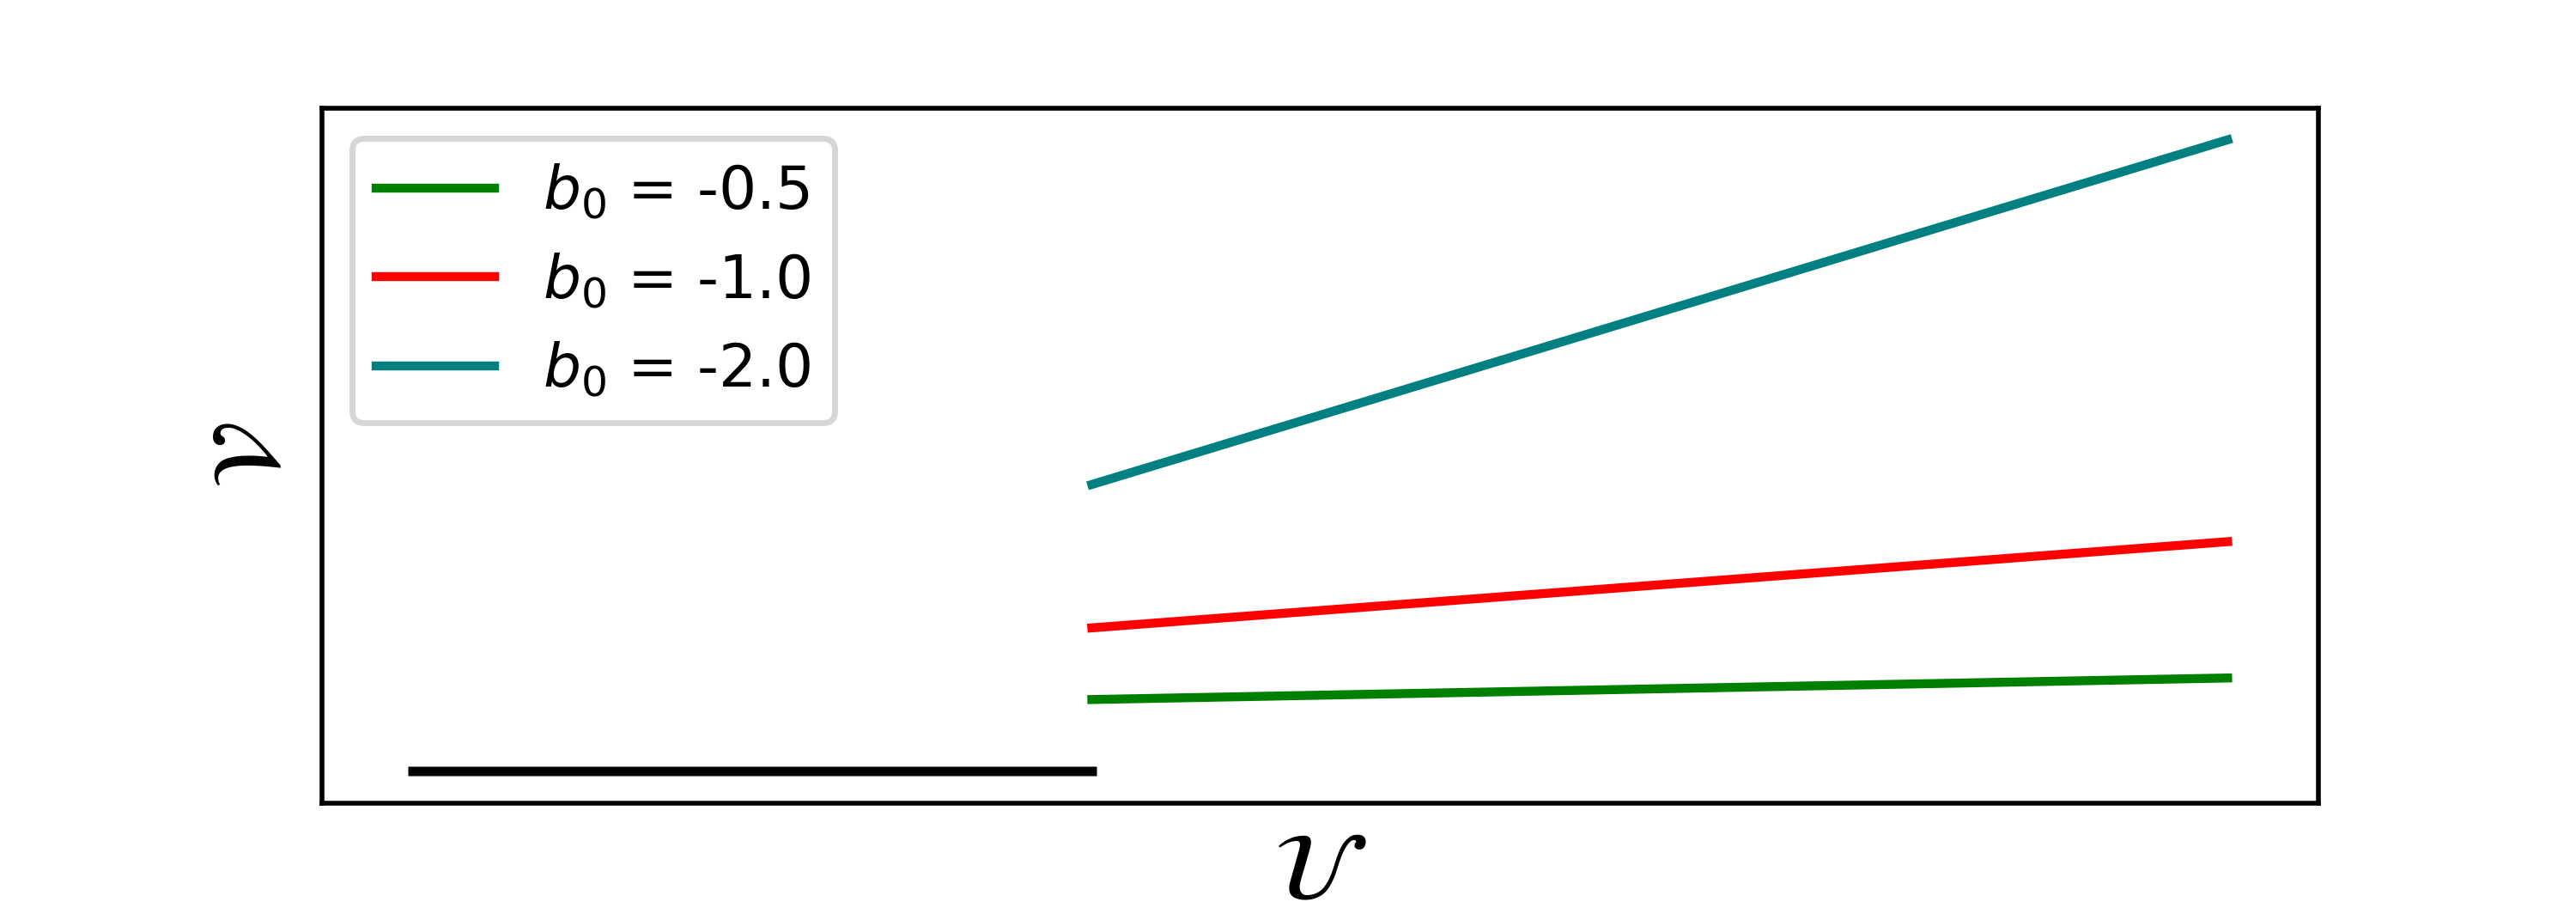
\includegraphics[width=.95\textwidth, clip]{../img/kap02/ASNullRing_UV.png}};
        \filldraw[white] (7.1,0.15) circle (10pt);
        \node[text width=12pt, anchor=north] at (7.1,0.5) {$\matu$};
        \filldraw[white] (1.3,2.3) circle (11pt);
        \node[text width=12pt, anchor=north] at (1.4,2.6) {$\matv$};
        \draw[dashed, thick, gray] (5.84,0.58) -- (5.84,4.22);
    \end{tikzpicture}
     \caption{Nulové geodetiky ($\dot \matu^-=1$, $\dot \matv^-=0$, $\dot \eta^-=0$) procházející impulzem
     AS řešení v $\rho=2$ pro různé parametry $b_0$.}
     \label{fig:Null_UV_AichelburgSexl_parameters}
\end{figure}

\begin{figure}[ht]
    \centering
    \begin{subfigure}[b]{0.45\textwidth}
        \begin{tikzpicture}
            \node[inner sep=0pt, anchor=south west] (ds) at (0,0)
            {\adjincludegraphics[trim={{.1\width} {.15\height} {.1\width} {.25\height}}, width=\textwidth, clip]{../img/kap02/ASNullRingxyUmu-1.pdf}};
            \filldraw[white] (0.59,2.65) circle (5pt);
            \node[text width=7pt] at (0.59,2.65) {\footnotesize{$\matu$}};
            \filldraw[white] (1.83,0.55) circle (5pt);
            \node[text width=7pt] at (1.82,0.55) {\footnotesize{$y$}};
            \filldraw[white] (4.7,0.55) circle (5pt);
            \node[text width=7pt] at (4.7,0.55) {\footnotesize{$x$}};
        \end{tikzpicture}
        \caption{$b_0 = -1$}
    \end{subfigure}
    \hfill
    \begin{subfigure}[b]{0.45\textwidth}
        \begin{tikzpicture}
            \node[inner sep=0pt, anchor=south west] (ds) at (0,0)
            {\adjincludegraphics[trim={{.1\width} {.15\height} {.1\width} {.25\height}}, width=\textwidth, clip]{../img/kap02/ASNullRingxyUmu-2.pdf}};
            \filldraw[white] (0.59,2.65) circle (5pt);
            \node[text width=7pt] at (0.59,2.65) {\footnotesize{$\matu$}};
            \filldraw[white] (1.83,0.55) circle (5pt);
            \node[text width=7pt] at (1.82,0.55) {\footnotesize{$y$}};
            \filldraw[white] (4.7,0.55) circle (5pt);
            \node[text width=7pt] at (4.7,0.55) {\footnotesize{$x$}};
        \end{tikzpicture}
        \caption{$b_0 = -2$}
    \end{subfigure}
    \caption{Nulové geodetiky ($\dot \matu^-=1$, $\dot \matv^-=0$, $\dot \eta^-=0$) procházející impulzní vlnou Aichelburg--Sexlova řešení. Prstenec testovacích částic je před průchodem impulzem v $\rho=2$.}
    \label{fig:NullASRing01}
\end{figure}

Záporné hodnoty parametru $b_0$, použté na obrázcích \ref{fig:Null_UV_AichelburgSexl_parameters} a \ref{fig:NullASRing01}, byly vhodné pro přehlednější vizualizaci
efektu impulzní vlny, nemají ale v originální konstrukci Aichelburg-Sexlova ultraboostu fyzikální význam. Parametr $b_0$
představuje v ultraboostové limitě $v \to 1, m \to 0$ konstantu, která splňuje $8m = b_0\sqrt{1-v^2}$, pro fyzikální systémy konstruované touto metodou
tedy nabývá kladných hodnot. Příklady nulových geodetiky pro kladné hodnoty jsou na obrázku \ref{fig:ASNullFyzikalnejsi}, kde vidíme,
že geodetiky jsou refraktovány směrem k $\rho=0$ -- jde tedy o přitažlivý efekt nulové částice generující impulzní vlnu.

\begin{figure}[ht]
    \centering
    \begin{subfigure}[b]{0.45\textwidth}
        \begin{tikzpicture}
            \node[inner sep=0pt, anchor=south west] (ds) at (0,0)
            {\adjincludegraphics[trim={{.1\width} {.1\height} {.1\width} {.25\height}}, width=\textwidth, clip]{../img/kap02/ASNullRingxyUmu1.pdf}};
            \filldraw[white] (0.59,3.1) circle (5pt);
            \node[text width=7pt] at (0.59,3.1) {\footnotesize{$\matu$}};
            \filldraw[white] (1.83,0.87) circle (5pt);
            \node[text width=7pt] at (1.82,0.87) {\footnotesize{$y$}};
            \filldraw[white] (4.7,0.85) circle (5pt);
            \node[text width=7pt] at (4.7,0.85) {\footnotesize{$x$}};
        \end{tikzpicture}
        \caption{$b_0 = 1$}
    \end{subfigure}
    \hfill
    \begin{subfigure}[b]{0.45\textwidth}
        \begin{tikzpicture}
            \node[inner sep=0pt, anchor=south west] (ds) at (0,0)
            {\adjincludegraphics[trim={{.1\width} {.1\height} {.1\width} {.25\height}}, width=\textwidth, clip]{../img/kap02/ASNullRingxyUmu2.pdf}};
            \filldraw[white] (0.59,3.1) circle (5pt);
            \node[text width=7pt] at (0.59,3.1) {\footnotesize{$\matu$}};
            \filldraw[white] (1.83,0.87) circle (5pt);
            \node[text width=7pt] at (1.82,0.87) {\footnotesize{$y$}};
            \filldraw[white] (4.7,0.85) circle (5pt);
            \node[text width=7pt] at (4.7,0.85) {\footnotesize{$x$}};
        \end{tikzpicture}
        \caption{$b_0 = 2$}
    \end{subfigure}
\caption{Nulové geodetiky ($\dot \matu^-=1$, $\dot \matv^-=0$, $\dot \eta^-=0$) procházející impulzem v $\rho=2$ pro kladné, tedy fyzikální hodnoty parametru $b_0$.}
\label{fig:ASNullFyzikalnejsi}
\end{figure}

Testovací částice s časupodobnými geodetikami se chovají stejným způsobem, na obrázku \ref{fig:AsMatter01} je vyobrazeno
šíření testovacích částic paralelně s osou $z$. Při průchodu $\matu = 0$ dochází k refrakci a částice po průchodu letí směrem k ose $z$.

\begin{figure}[ht]
    \centering
    \begin{subfigure}[b]{0.45\textwidth}
        \begin{tikzpicture}
            \node[inner sep=0pt, anchor=south west] (ds) at (0,0)
        {\adjincludegraphics[trim={{.1\width} {.15\height} {.1\width} {.25\height}}, width=\textwidth, clip]{../img/kap02/ASMatterRingxyUmu0.5.pdf}};
        \filldraw[white] (0.59,2.6) circle (5pt);
        \node[text width=7pt] at (0.59,2.6) {\footnotesize{$\matu$}};
        \filldraw[white] (1.83,0.56) circle (5pt);
        \node[text width=7pt] at (1.82,0.56) {\footnotesize{$y$}};
        \filldraw[white] (4.7,0.57) circle (5pt);
        \node[text width=7pt] at (4.7,0.57) {\footnotesize{$x$}};
        \end{tikzpicture}
        \caption{$b_0 = 0.5$}
    \end{subfigure}
    \hfill
    \begin{subfigure}[b]{0.45\textwidth}
        \begin{tikzpicture}
            \node[inner sep=0pt, anchor=south west] (ds) at (0,0)
            {\adjincludegraphics[trim={{.1\width} {.15\height} {.1\width} {.25\height}}, width=\textwidth, clip]{../img/kap02/ASMatterRingxyUmu2.pdf}};
            \filldraw[white] (0.59,2.6) circle (5pt);
            \node[text width=7pt] at (0.59,2.6) {\footnotesize{$\matu$}};
            \filldraw[white] (1.83,0.56) circle (5pt);
            \node[text width=7pt] at (1.82,0.56) {\footnotesize{$y$}};
            \filldraw[white] (4.7,0.57) circle (5pt);
            \node[text width=7pt] at (4.7,0.57) {\footnotesize{$x$}};
        \end{tikzpicture}
        \caption{$b_0 = 2$}
    \end{subfigure}
    \caption{Časupodobné geodetiky ($\dot \matu^-=\frac{1}{2}$, $\dot \matv^-=1$, $\dot \eta^-=0$) procházející impulzní vlnou AS řešení. Prstenec testovacích částic je před průchodem impulzem lokalizován v $\rho=2$.}
    \label{fig:AsMatter01}
\end{figure}

Refrakce je slabší s rostoucí vzdáleností od částice generující impulz. Na obrázku \ref{fig:AS_zavislost_na_rho} jsou znázorněny už
refraktované časupodobné geodetiky pro různé vzdálenosti od osy symetrie. Před refrakcí se jedná o pohyb testovacích částic ve směru osy $z$.
Takové chování odpovídá intuitivnímu očekávání při uvážení fyzikální podstaty zdroje v AS řešení.

\begin{figure}[!ht]
    \centering
       \begin{tikzpicture}
           \node[inner sep=0pt, anchor=south west] (ds) at (0,0)
           {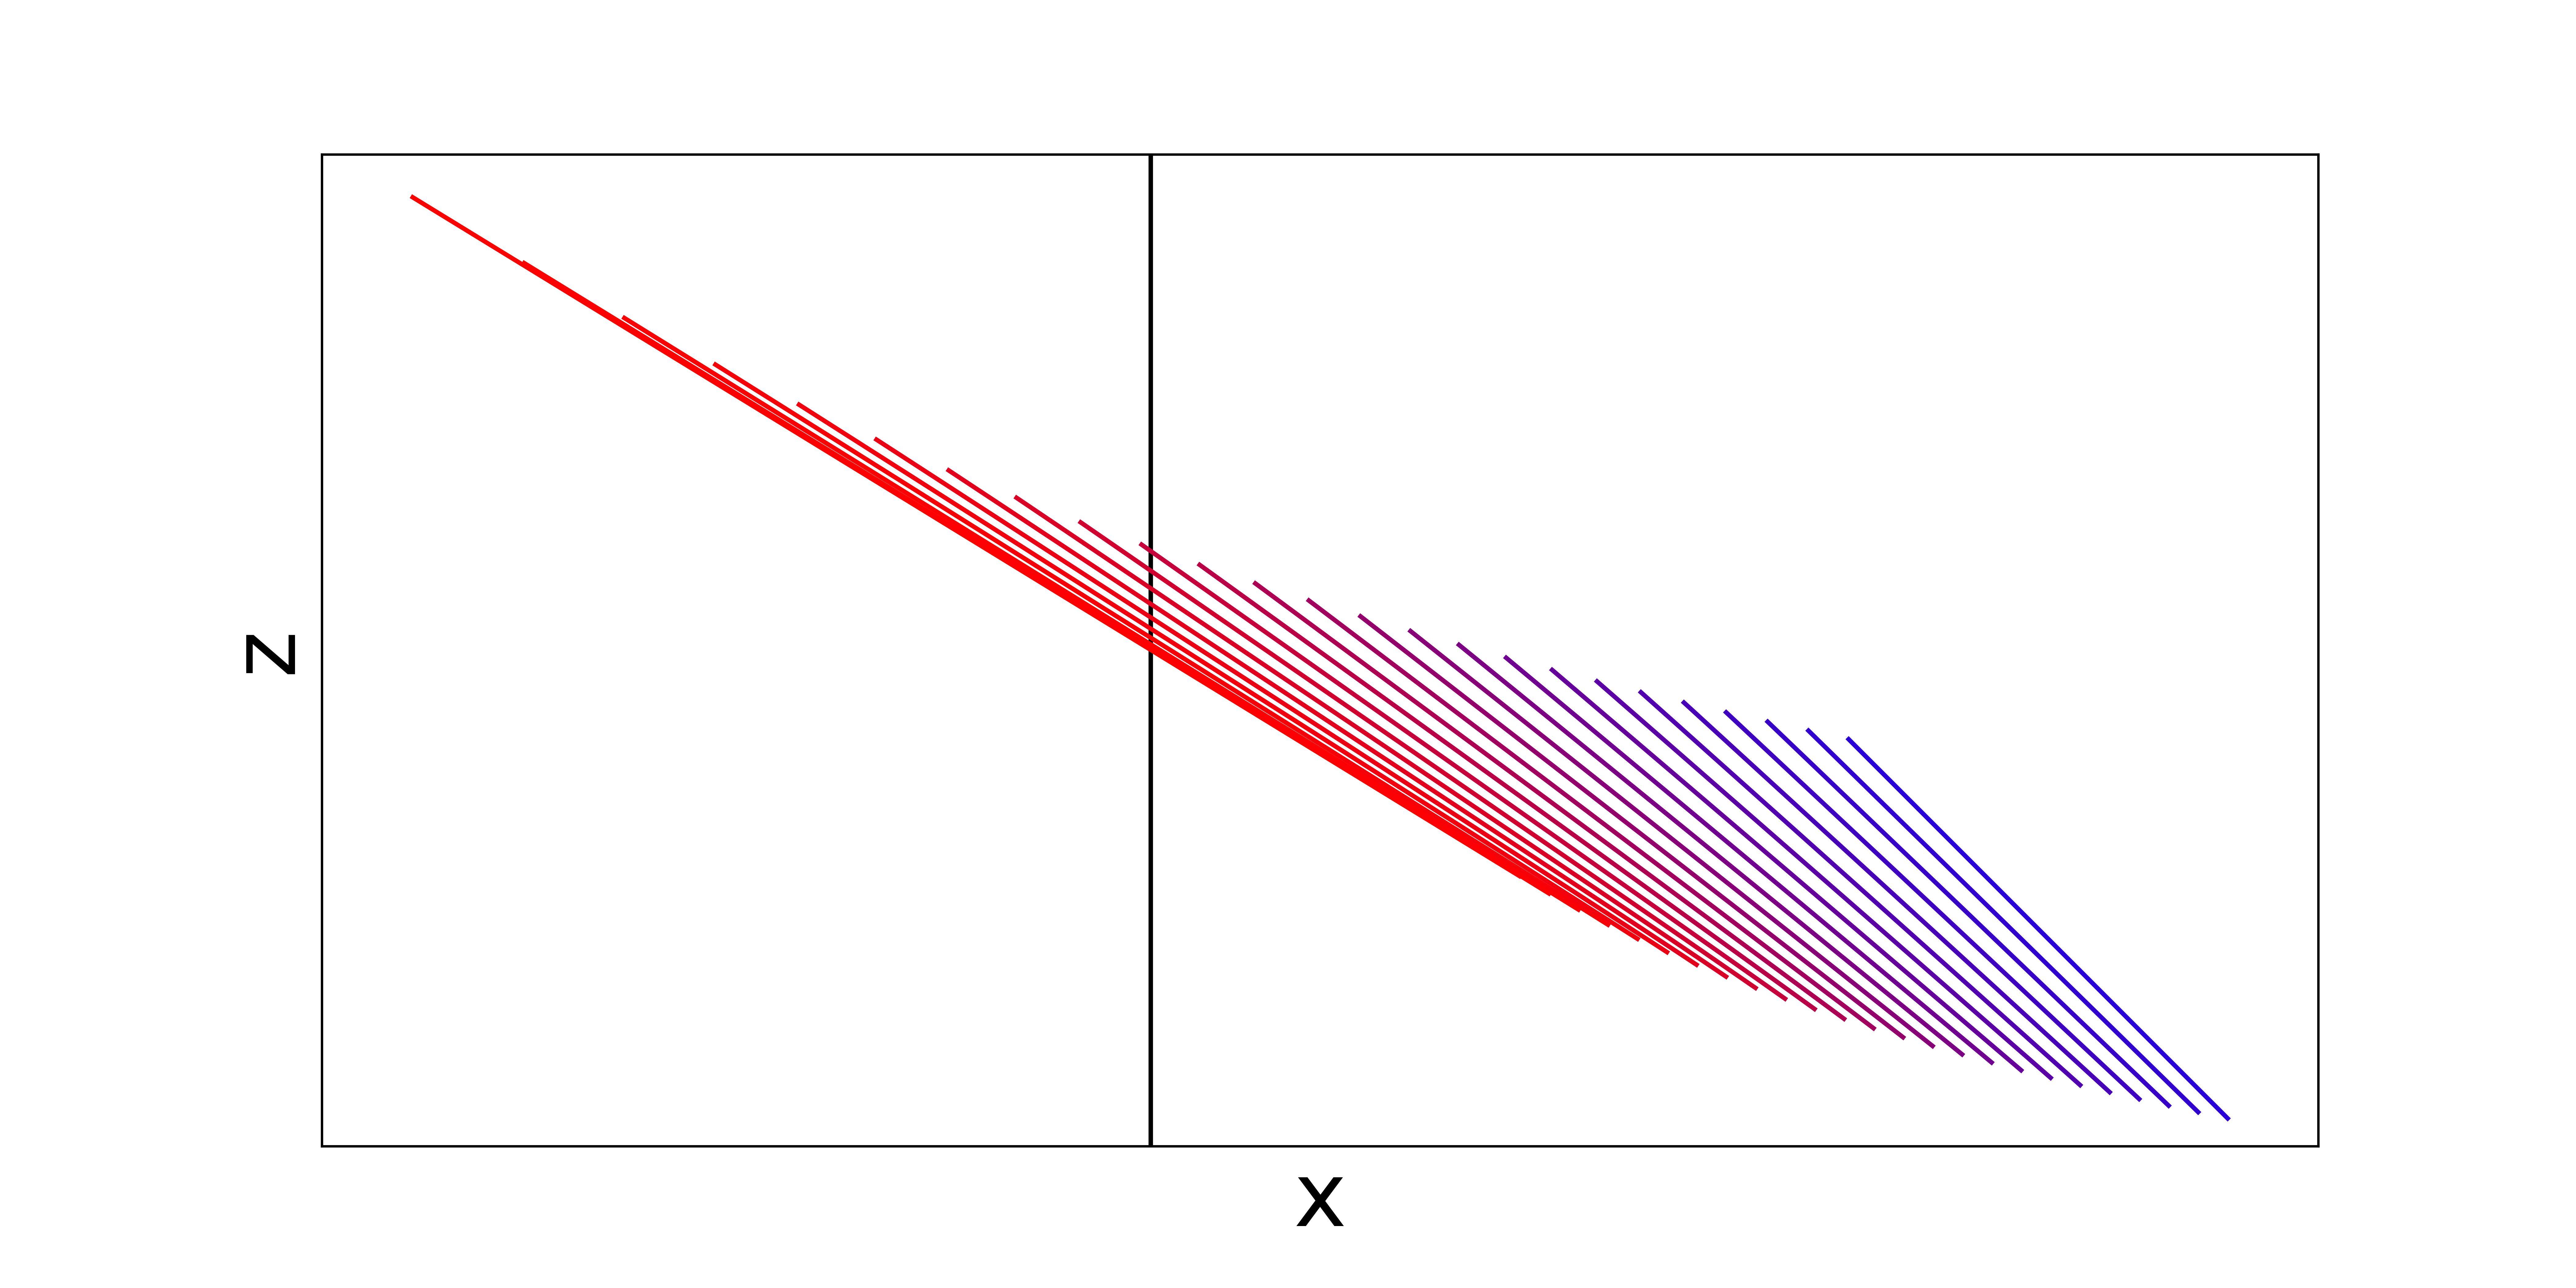
\includegraphics[width=.7\textwidth, clip]{../img/kap02/ASMatterLinexz.png}};
           \filldraw[white] (5.2,0.15) circle (9pt);
            \node[text width=10pt] at (5.2,0.15) {$x$};
            \filldraw[white] (0.9,2.4) circle (9pt);
            \node[text width=10pt] at (1,2.4) {$z$};
        \end{tikzpicture}
    \caption{Refraktované časupodobné geodetiky po průchodu impulzem v různých vzdálenostech $\rho$ pro $b_0 = \frac{1}{2}$.
    Červená barva odpovídá částici refraktované nejblíže ($\rho=\frac{1}{2}$), modrá nejdále ($\rho = 2$). Černá přímka odpovídá
    ose $x=0$.}
    \label{fig:AS_zavislost_na_rho}
\end{figure}


Pro potěšení oka čtenáře jsou přiloženy další vizualizace geodetického pohybu v Aichelburg-Sexlově řešení. Na obrázku \ref{fig:AsMatter02} je systém časupodobných geodetik, které se před
průchodem impulzní vlnou šíří směrem od osy symetrie $z$. V (b) dochází k refrakci, která otáčí směr šíření směrem zpět k ose $z$.
Na obrázku \ref{fig:AsMatterNonAxial} je pak zobrazení průchodu geodetik, které nejsou uspořádány axiálně symetricky.

\begin{figure}[ht]
    \centering
    \begin{subfigure}[b]{0.45\textwidth}
        \begin{tikzpicture}
            \node[inner sep=0pt, anchor=south west] (ds) at (0,0)
            {\adjincludegraphics[trim={{.1\width} {.15\height} {.1\width} {.25\height}}, width=\textwidth, clip]{../img/kap02/ASMatterRing_XYMOVING__xyU_mu2.pdf}};
            \filldraw[white] (0.59,2.7) circle (5pt);
            \node[text width=7pt] at (0.59,2.7) {\footnotesize{$\matu$}};
            \filldraw[white] (1.83,0.54) circle (5pt);
            \node[text width=7pt] at (1.82,0.54) {\footnotesize{$y$}};
            \filldraw[white] (4.7,0.57) circle (5pt);
            \node[text width=7pt] at (4.7,0.57) {\footnotesize{$x$}};
        \end{tikzpicture}
        \caption{$b_0 = 2$}
    \end{subfigure}
    \hfill
    \begin{subfigure}[b]{0.45\textwidth}
        \begin{tikzpicture}
            \node[inner sep=0pt, anchor=south west] (ds) at (0,0)
            {\adjincludegraphics[trim={{.1\width} {.15\height} {.1\width} {.25\height}}, width=\textwidth, clip]{../img/kap02/ASMatterRing_XYMOVING__xyU_mu4.pdf}};
            \filldraw[white] (0.59,2.7) circle (5pt);
            \node[text width=7pt] at (0.59,2.7) {\footnotesize{$\matu$}};
            \filldraw[white] (1.83,0.54) circle (5pt);
            \node[text width=7pt] at (1.82,0.54) {\footnotesize{$y$}};
            \filldraw[white] (4.7,0.57) circle (5pt);
            \node[text width=7pt] at (4.7,0.57) {\footnotesize{$x$}};
        \end{tikzpicture}
        \caption{$b_0 = 4$}
    \end{subfigure}
    \caption{Časupodobné geodetiky ($\dot \matu^-=1$, $\dot \matv^-=2$, $\dot \eta^-=\sqrt{\frac{3}{2}} e^{i \phi}$), kde $\phi$ odpovídá úhlu v
    cylindrických souřadnicích, ve kterém částice leží, procházející impulzní vlnou AS řešení v $\rho=2$.}
    \label{fig:AsMatter02}
\end{figure}

\begin{figure}[ht]
    \centering
    \begin{tikzpicture}
        \node[inner sep=0pt, anchor=south west] (ds) at (0,0)
        {\adjincludegraphics[trim={{.1\width} {.15\height} {.1\width} {.22\height}}, width=0.8\textwidth, clip]{../img/kap02/ASMatterHearthxyUmu1.pdf}};
        \filldraw[white] (1.87,2.7) circle (9pt);
        \node[text width=9pt] at (1.87,2.7) {\small{$\matu$}};
        \filldraw[white] (8.8,2.7) circle (10pt);
        \node[text width=7pt] at (8.8,2.7) {\small{$y$}};
        \filldraw[white] (5,0.57) circle (10pt);
        \node[text width=7pt] at (5,0.57) {\small{$x$}};
    \end{tikzpicture}
    \caption{Časupodobné geodetiky ($\dot \matu^-=\frac{1}{2}$, $\dot \matv^-=1$, $\dot \eta^-=0$) ve vybraném uspořádání procházející nadplochou $\matu = 0$.}
    \label{fig:AsMatterNonAxial}
\end{figure}
Pro $m>0$ závisí změna geodetického pohybu na prostorovém úhlu. Derivace profilové funkce $H_{i,Z}$, která vystupuje v refrakčních rovnicích, je pro jednotlivá $m$
\begin{equation}
    H_{i,Z}^{(m)}(\eta, \bar{\eta}) = -\frac{(\sqrt{2})^{m} b_m m}{\eta^{m+1}}.
\end{equation}
Speciálně pro $m=1$, tedy impulz generovaný částicí s dipólovou strukturou, je $H_{i,Z}^{(1)}$ vykreslena na obrázku \ref{fig:DipoleHZ}. Reálná část a imaginární část
odpovídá derivacím ve směru $X$ a $Y$ vystupujícím v refrakčních rovnicích \eqref{eq:refraction_velocity_null_cart} - přímo tedy ukazují závislost změny čtyřrychlosti v těchto směrech na místě průchodu geodetiky vlnoplochou,

\begin{equation}
    \begin{split}
        Re(H_{i,Z}) &= \frac{1}{\sqrt{2}} H_{i,X}, \\
        Im(H_{i,Z}) &=-\frac{1}{\sqrt{2}}H_{i,Y}.
    \end{split}
\end{equation}


Příklad nulových geodetik procházejících impulzem s jediným nenulovým členem pro $m=1$ je na obrázku \ref{fig:DipoleAxial}, pro časupodobné geodetiky dostáváme totožné
chování (viz obrázek \ref{fig:DipoleAxialTimelike})

\begin{figure}[ht]
    \centering
    \begin{subfigure}[b]{0.45\textwidth}
        \begin{tikzpicture}
            \node[inner sep=0pt, anchor=south west] (ds) at (0,0)
        {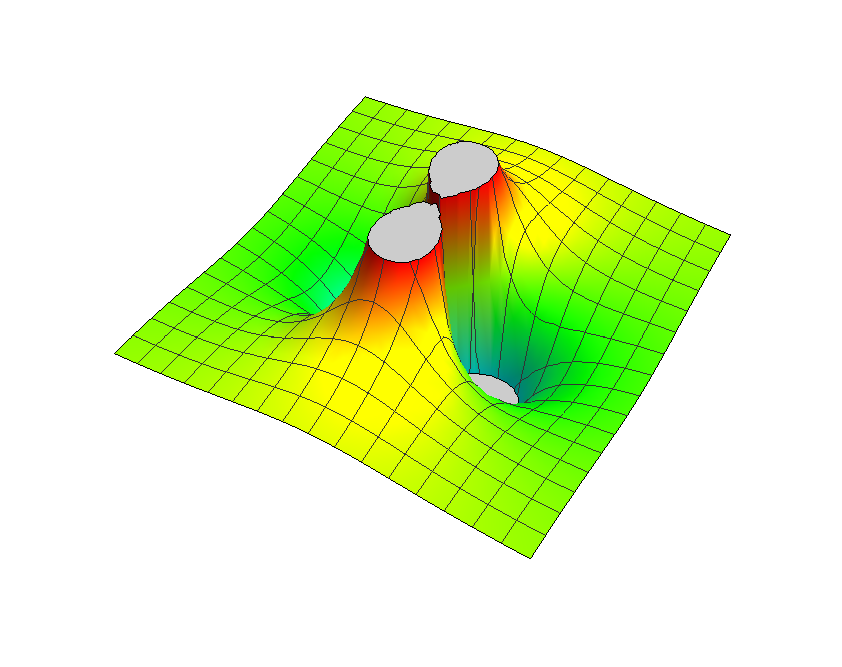
\includegraphics[width=1\textwidth, clip]{../img/kap02/DipoleHZReal.pdf}};
        \end{tikzpicture}
        \caption{$\Re(H_{i,Z}^{(1)})$}
    \end{subfigure}
    \hfill
    \begin{subfigure}[b]{0.45\textwidth}
        \begin{tikzpicture}
            \node[inner sep=0pt, anchor=south west] (ds) at (0,0)
            {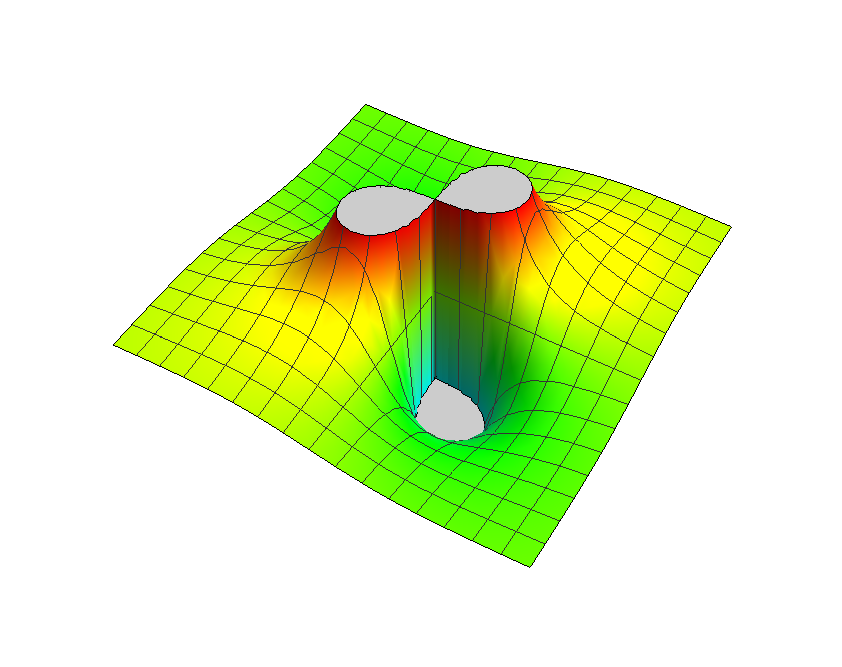
\includegraphics[width=1\textwidth, clip]{../img/kap02/DipoleHZImaginary.pdf}};
        \end{tikzpicture}
        \caption{$\Im(H_{i,Z}^{(1)})$}
    \end{subfigure}
    \caption{Reálná a imaginární část funkce profilu vlny $H_{i,Z}^{(1)}(x, y)$.}
    \label{fig:DipoleHZ}
\end{figure}
\begin{figure}[ht]
    \centering
    \begin{tikzpicture}
        \node[inner sep=0pt, anchor=south west] (ds) at (0,0)
        {\adjincludegraphics[trim={{.1\width} {.15\height} {.1\width} {.22\height}}, width=0.8\textwidth, clip]{../img/kap02/DipoleNullxyUb1_0.2.pdf}};
        \filldraw[white] (9.2,2) circle (9pt);
        \node[text width=9pt] at (9.2,2) {\small{$\matu$}};
        \filldraw[white] (2,4.92) circle (6pt);
        \node[text width=7pt] at (2,4.92) {\small{$x$}};
        \node at (5.8,1.083) [rectangle,draw, white, fill=white] {$y$};
        \node[text width=7pt] at (5.8,1.13) {\small{$y$}};
    \end{tikzpicture}    
    \caption{Nulové geodetiky ($\dot \matu^-=1$, $\dot \matv^-=0$, $\dot \eta^-=0$) v axiálně symetrickém uspořádání ($\rho=1$) na $\mathcal{M}^-$ procházející impulzní nadplochou vlny generované částicí s dipólovou strukturou
    s parametrem $b_1=0.2$.}
    \label{fig:DipoleAxial}
\end{figure}
\begin{figure}[ht]
    \centering
    \begin{tikzpicture}
        \node[inner sep=0pt, anchor=south west] (ds) at (0,0)
        {\adjincludegraphics[trim={{.1\width} {.15\height} {.1\width} {.22\height}}, width=0.8\textwidth, clip]{../img/kap02/DipoleTimelikexyUb1_0.4.pdf}};
        \filldraw[white] (9.2,2) circle (9pt);
        \node[text width=9pt] at (9.2,2) {\small{$\matu$}};
        \filldraw[white] (2,4.92) circle (6pt);
        \node[text width=7pt] at (2,4.92) {\small{$x$}};
        \node at (5.8,1.083) [rectangle,draw, white, fill=white] {$y$};
        \node[text width=7pt] at (5.8,1.13) {\small{$y$}};
    \end{tikzpicture}    
    \caption{Časupodobné geodetiky ($\dot \matu^-=0.5$, $\dot \matv^-=1$, $\dot \eta^-=0$) v axiálně symetrickém uspořádání ($\rho=1$) na $\mathcal{M}^-$ procházející impulzní nadplochou vlny generované částicí s dipólovou strukturou,
    s parametrem $b_1=0.4$.}
    \label{fig:DipoleAxialTimelike}
\end{figure}
\clearpage

\subsection{Impulzní gravitační vlna generovaná nehmotnými částicemi s multipólovou strukturou s \texorpdfstring{$\Lambda\neq 0$}{Lambda =/= 0}}

V prostoročasech s nenulovou konstantou odvodili Griffiths a Podolský \cite{Podolsky1997} tvar řešení obdobný \eqref{eq:multipole_minkowski},
tedy případ impulzních vln generovaných nulovými částicemi s multipólovou strukturou. Vyšli z redukce Einsteinových rovnic pro distribuční
metriku \eqref{eq:5DDistributionalWaveMetric}. V případě ryze gravitačních vln dostáváme podmínku
\begin{equation}
    \label{eq:podminka_na_H_lambda_stare}
    \left(\Delta + \frac{2}{3} \Lambda \right)\mathcal{H} = 0,
\end{equation}
kde $\Delta$ je Laplaceův operátor působící na impulzní nadploše. Při parametrizaci 
\begin{equation}
    \begin{split}
        Z_2 &= a \sqrt{\epsilon(1-z^2)} \cos \phi,\\
        Z_3 &= a \sqrt{\epsilon(1-z^2)} \sin \phi,\\
        Z_4 &= a~z,
    \end{split}
\end{equation}
kde pro $\Lambda > 0$ je $\left|z\right| \leq 1$ a pro $\Lambda < 0$ je $\left|z\right| \geq 1$,
nabývá funkce $\mathcal{H}(z, \phi)$ tvaru
\begin{equation}
    \mathcal{H}(z, \phi) = b_0 Q_1(z) + \sum_{m=1}^\infty b_0 Q_1^m(z) \cos [m(\phi - \phi_m)],
\end{equation}
kde $Q_1^m(z)$ jsou přidružené Legendrovy funkce druhého druhu, tedy
\begin{equation}
    Q_1^m(z) = -(\epsilon)^m |1-z^2|^{m/2} \frac{d^m}{dz^m}Q_1(z).
\end{equation}

První člen
\begin{equation}
    b_0 Q_1(z) = b_0 \left(\frac{z}{2} \log \left|\frac{1+z}{1-z}\right| - 1\right)
\end{equation}
představuje axiálně symetrické Hottovo--Tanakovo řešení \cite{Hotta_1993}, které odpovídá boostu Schwarzschildova--(anti--)de Sitterova
prostoročasu. Toto řešení je analogií Aichelburg--Sexlova řešení v (anti--)de Sitterově prostoročasu se singulární hmotou generující vlnu v $z=1$. V případě de Sitterova prostoročasu je impulzní nadplocha
neexpandující sféra generovaná dvěma nehmotnými částicemi, které letí v opačném směru. V anti--de Sitterově prostoročasu je impulzní nadplocha hyperboloidální
plochou generovaná částicí, která se (díky tomu, že se jedná o nakrytí $\mathbb{R}^4$ s topologií $\mathbb{S}^1 \times \mathbb{R}^3$) periodicky pohybuje mezi prostorovými nekonečny,
z jedné strany na druhou.

Na obrázku \ref{fig:funkceHhodnotyvADS} vidíme hodnoty funkce $\mathcal{H}(Z_2, Z_3, Z_4)$ Hottova--Tanakova řešení na vlnoploše v (A--)dS prostoročasu (s $|\Lambda | = 1$).

\begin{figure}[ht]
    \centering
    \begin{subfigure}[b]{0.45\textwidth}
        \begin{tikzpicture}
            \node[inner sep=0pt, anchor=south west] (ds) at (0,0)
        {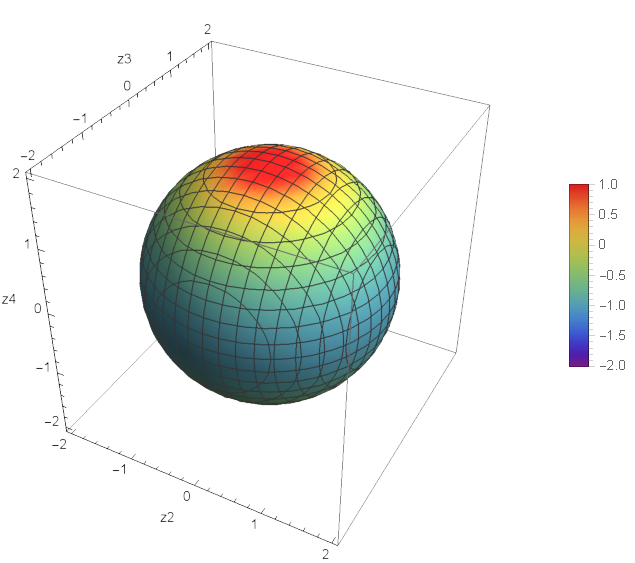
\includegraphics[width=1\textwidth, clip]{../img/kap02/dSWaveFrontHValue.pdf}};
        \end{tikzpicture}
        \caption{de Sitterův prostoročas}
    \end{subfigure}
    \hfill
    \begin{subfigure}[b]{0.45\textwidth}
        \begin{tikzpicture}
            \node[inner sep=0pt, anchor=south west] (ds) at (0,0)
            {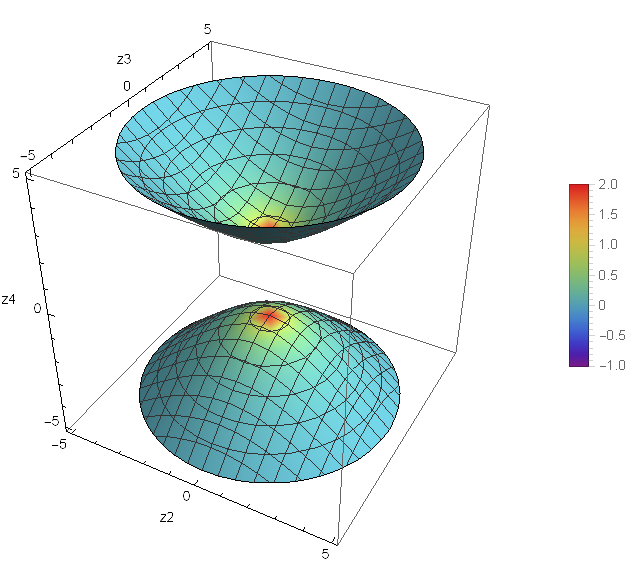
\includegraphics[width=1\textwidth, clip]{../img/kap02/AdSWaveFrontHValue.pdf}};
        \end{tikzpicture}
        \caption{anti--de Sitterův prostoročas}
    \end{subfigure}
    \caption{Funkce $\mathcal{H}$ má v de Sitterově prostoročasu singulární body na pólech sféry odpovídající vlnoploše ($Z_4 = \pm a$), v anti--de Sitterově
    prostoročase singularity leží na vrcholech hyperboloidálních vlnoploch.}
    \label{fig:funkceHhodnotyvADS}
\end{figure}

Geodetický pohyb nulových částic je v konformně plochých souřadnicích
nezávislý na hodnotě kosmologické konstanty, chování na impulzní ploše se pak liší pouze ve tvaru příslušné funkce $H(\eta, \bar{\eta})$, která má v případě Hottova--Tanakova řešení
v konformně plochých souřadnicích tvar
\begin{equation}
    \label{eq:Hotta_Tanaka_H_conf_flat_coords}
    H(\eta, \bar{\eta}) = \frac{1}{24} b_0 \left((\Lambda \eta \bar{\eta} + 6) \log \left(\left| \frac{6}{\Lambda \eta \bar{\eta} }\right| \right)+2 (\Lambda \eta \bar{\eta} - 6)\right),
\end{equation}
a v derivacích $H$ ve směru $\eta$, respektive $\bar{\eta}$.

Jako první ukážeme pohyb nulových částic v nadploše $y=0$ (to znamená, že souřadnice $\eta$ je reálná). Díky axiální symetrii tak zároveň prozkoumáme
vlastnosti nulových geodetik ve všech nadplochách obsahujících osu této symetrie.
Tento pohyb je pro řešení s $b_0 = 1$ zobrazen v konformně plochých souřadnicích  na obrázku \ref{fig:HottaTanakaNullY0}.

\begin{figure}[ht]
    \centering
    \begin{subfigure}[b]{0.45\textwidth}
        \begin{tikzpicture}
            \node[inner sep=0pt, anchor=south west] (ds) at (0,0)
            {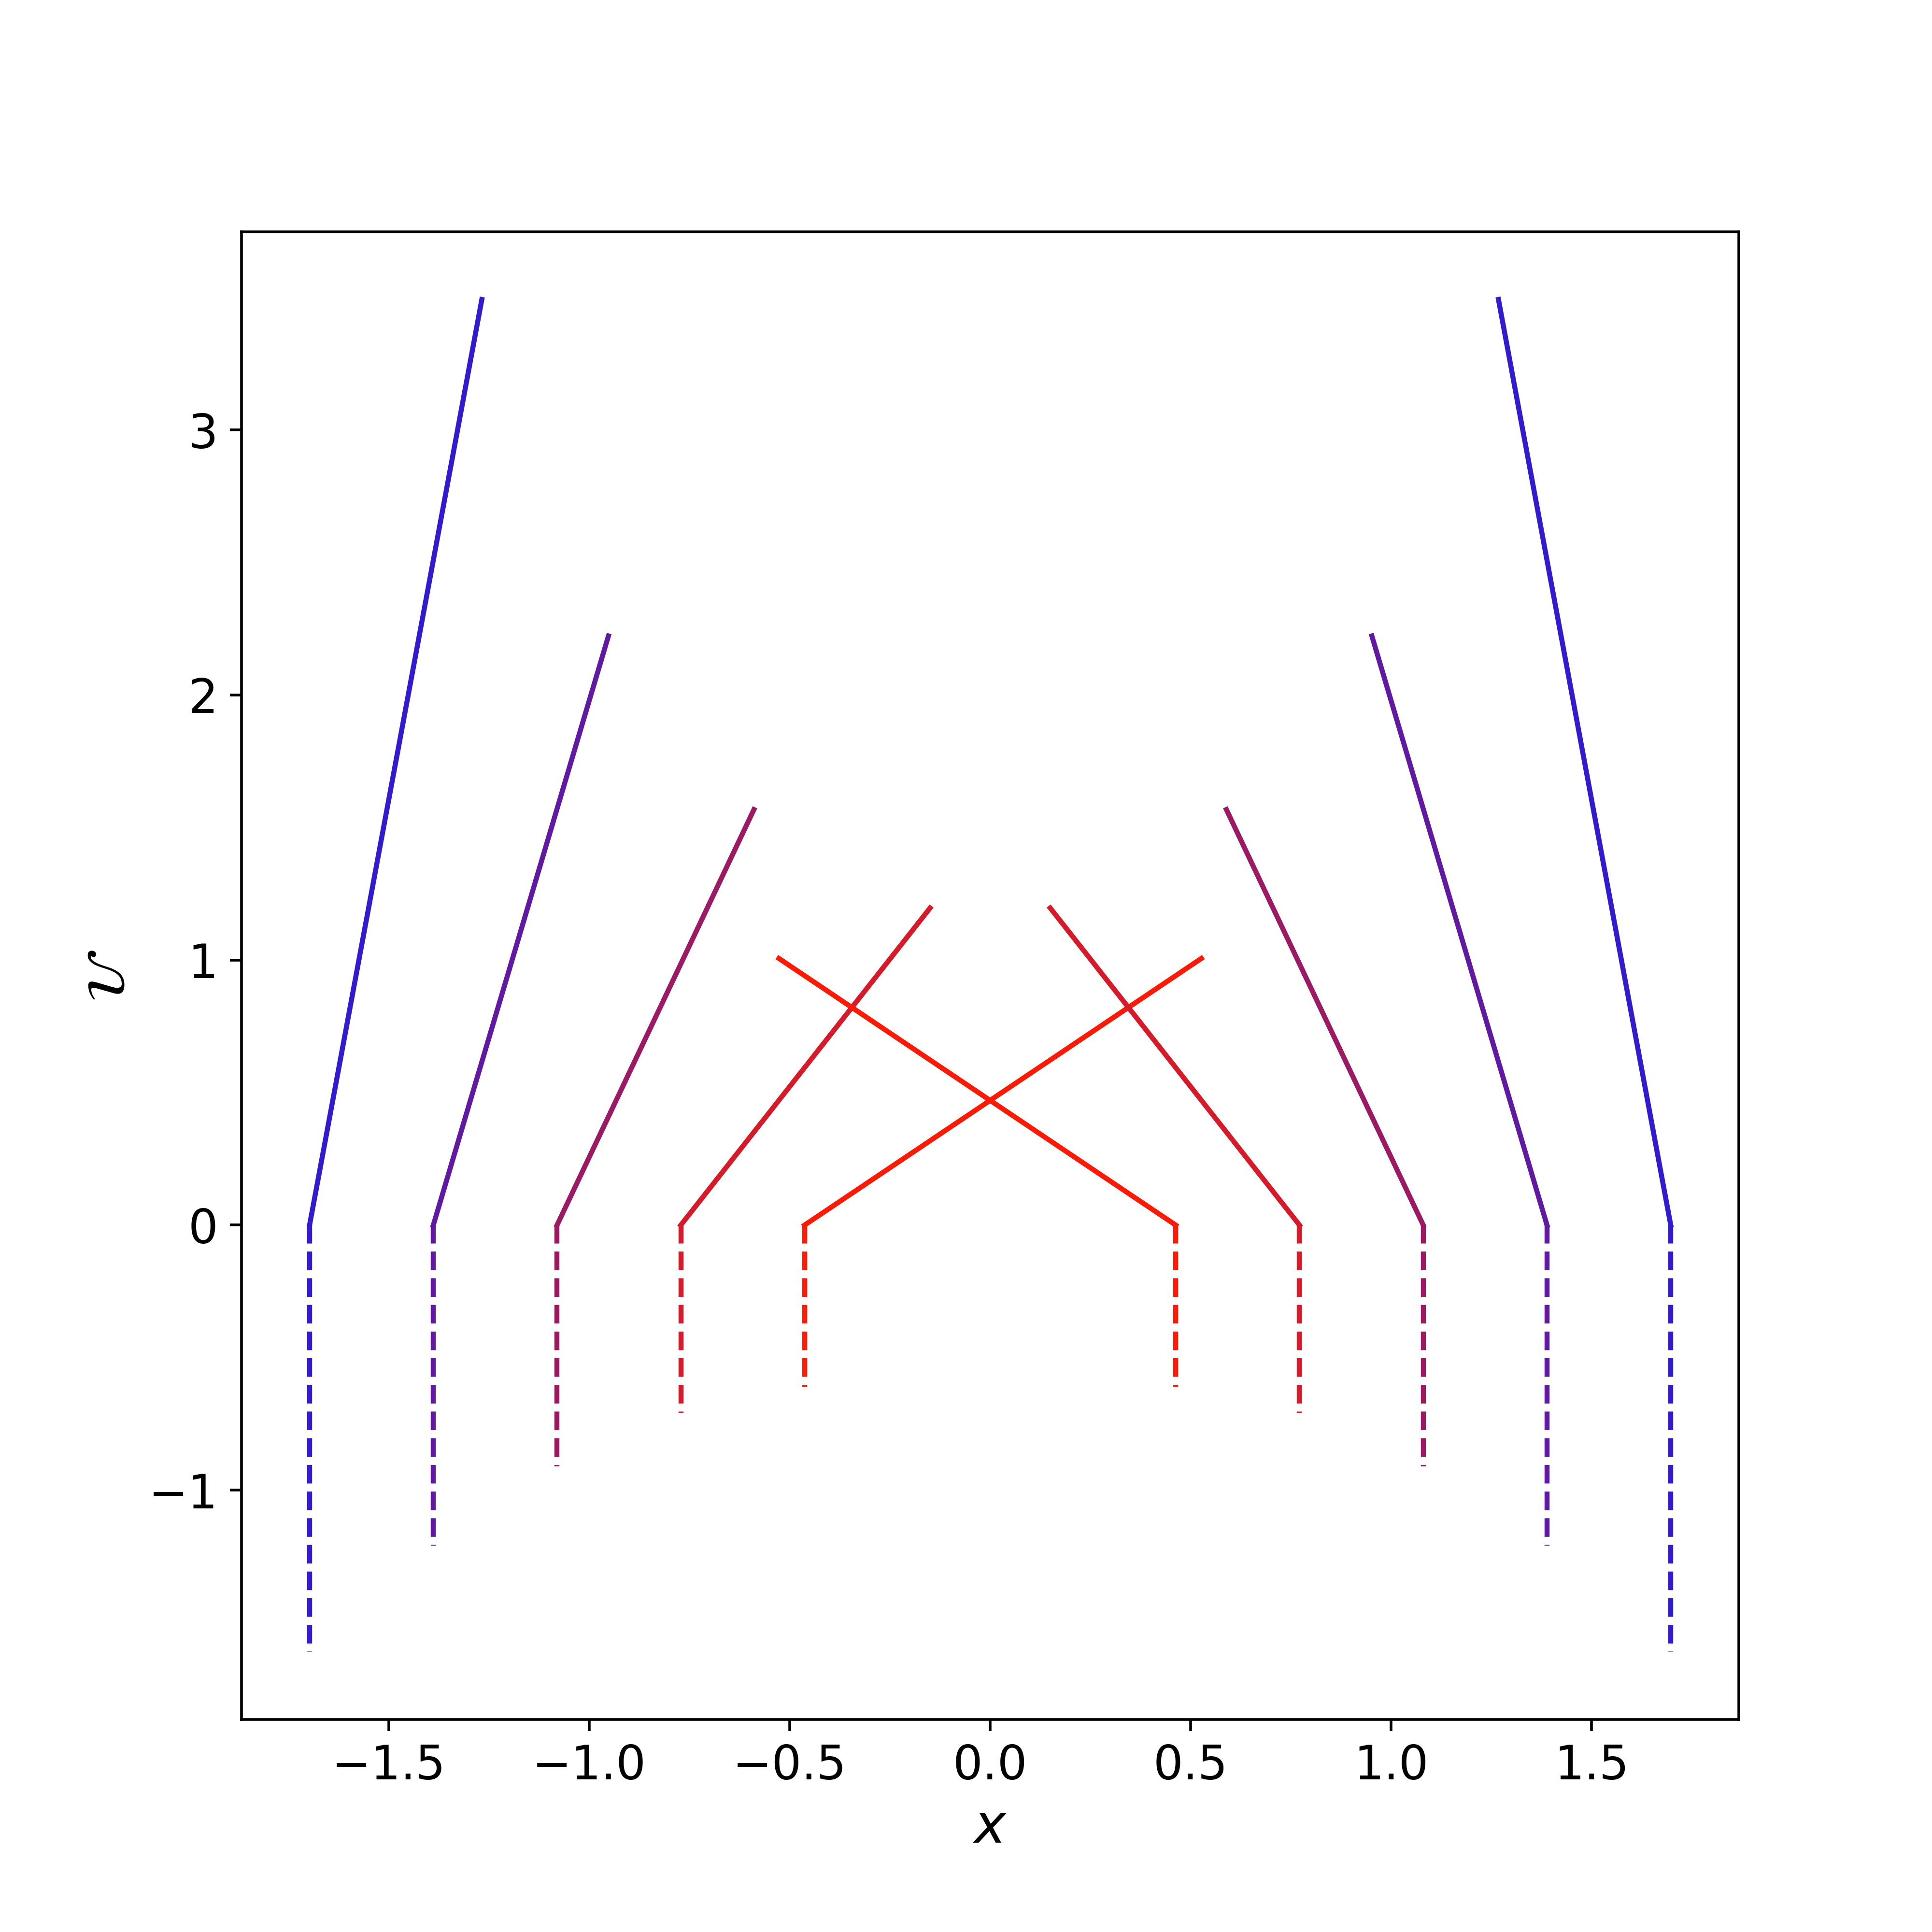
\includegraphics[width=.95\textwidth, clip]{../img/kap02/HT_y-0__xU_mu1_lmb1.png}};
            \filldraw[white] (0.29,3.1) circle (4pt);
            \node[text width=7pt] at (0.29,3.1) {\scriptsize{$\matu$}};
            \filldraw[white] (3.25,0.28) circle (4pt);
            \node[text width=7pt] at (3.25,0.28) {\scriptsize{$x$}};
        \end{tikzpicture}
        \caption{$\Lambda = 1$}
    \end{subfigure}
    \hfill
    \begin{subfigure}[b]{0.45\textwidth}
        \begin{tikzpicture}
            \node[inner sep=0pt, anchor=south west] (ds) at (0,0)
            {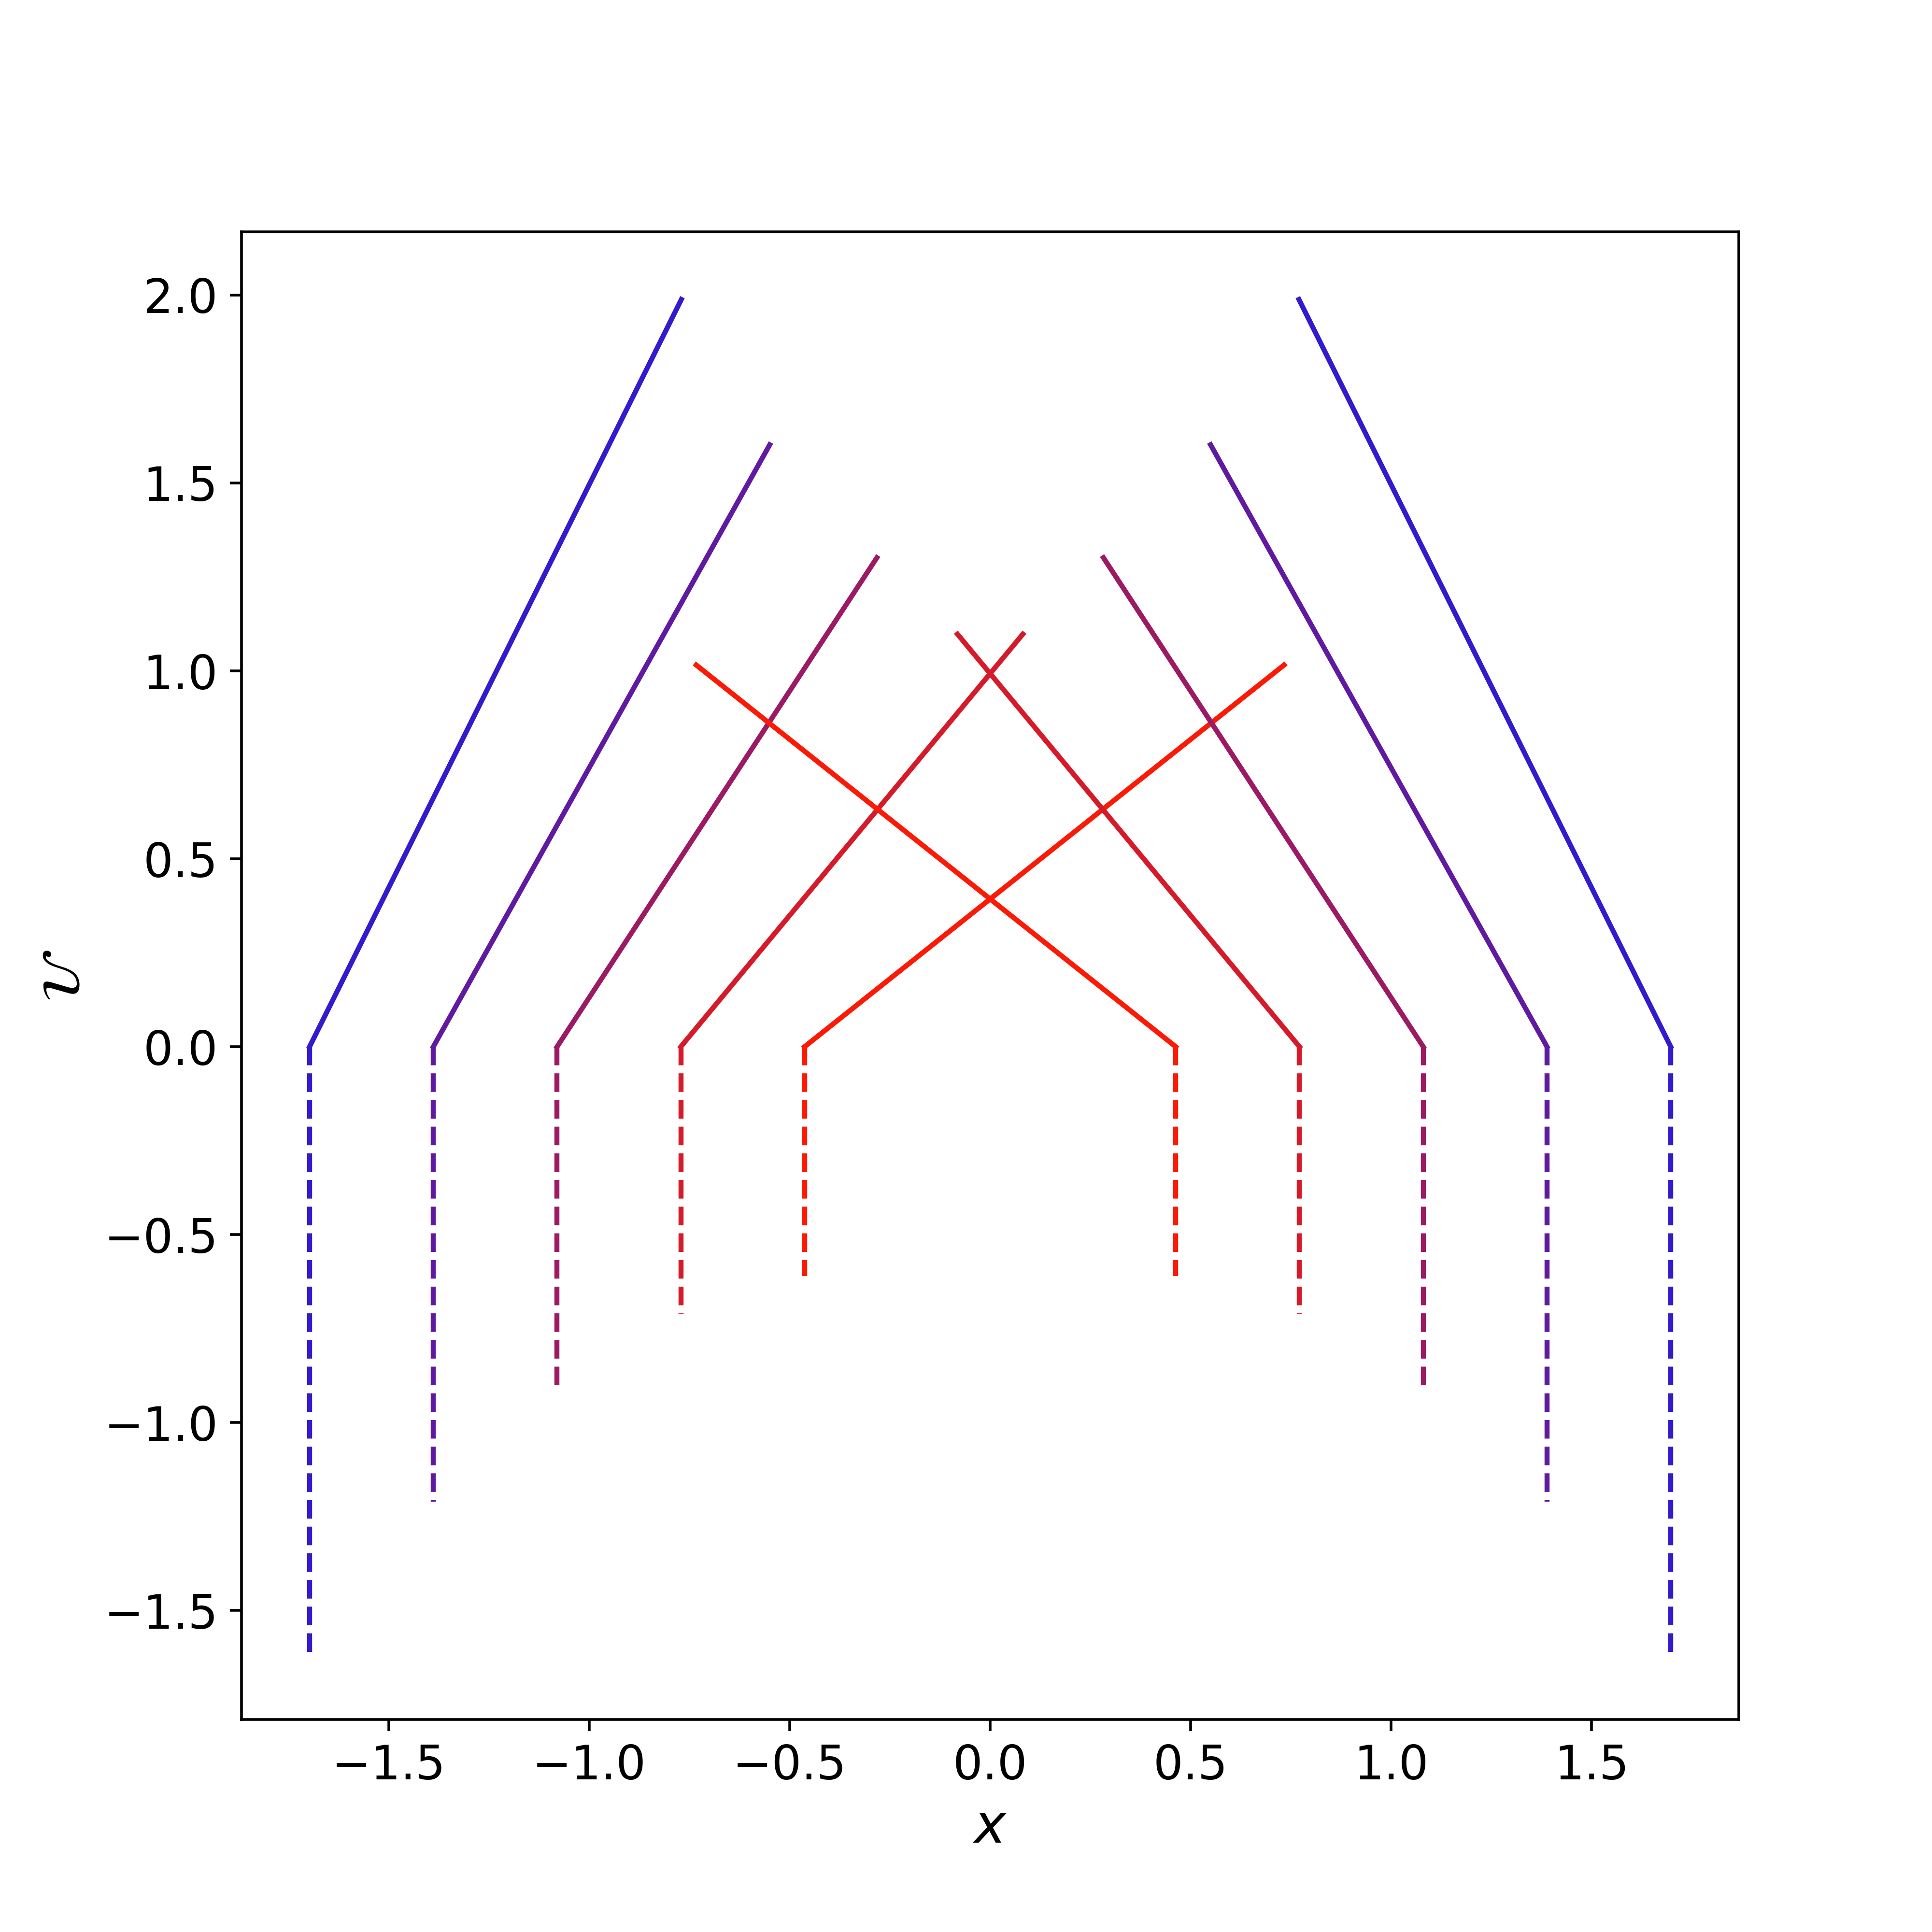
\includegraphics[width=.95\textwidth, clip]{../img/kap02/HT_y-0__xU_mu1_lmb-1.png}};
            \filldraw[white] (0.29,3.1) circle (4pt);
            \node[text width=7pt] at (0.29,3.1) {\scriptsize{$\matu$}};
            \filldraw[white] (3.25,0.28) circle (4pt);
            \node[text width=7pt] at (3.25,0.28) {\scriptsize{$x$}};
        \end{tikzpicture}
        \caption{$\Lambda = -1$}
    \end{subfigure}

    \begin{subfigure}[b]{0.45\textwidth}
        \begin{tikzpicture}
            \node[inner sep=0pt, anchor=south west] (ds) at (0,0)
            {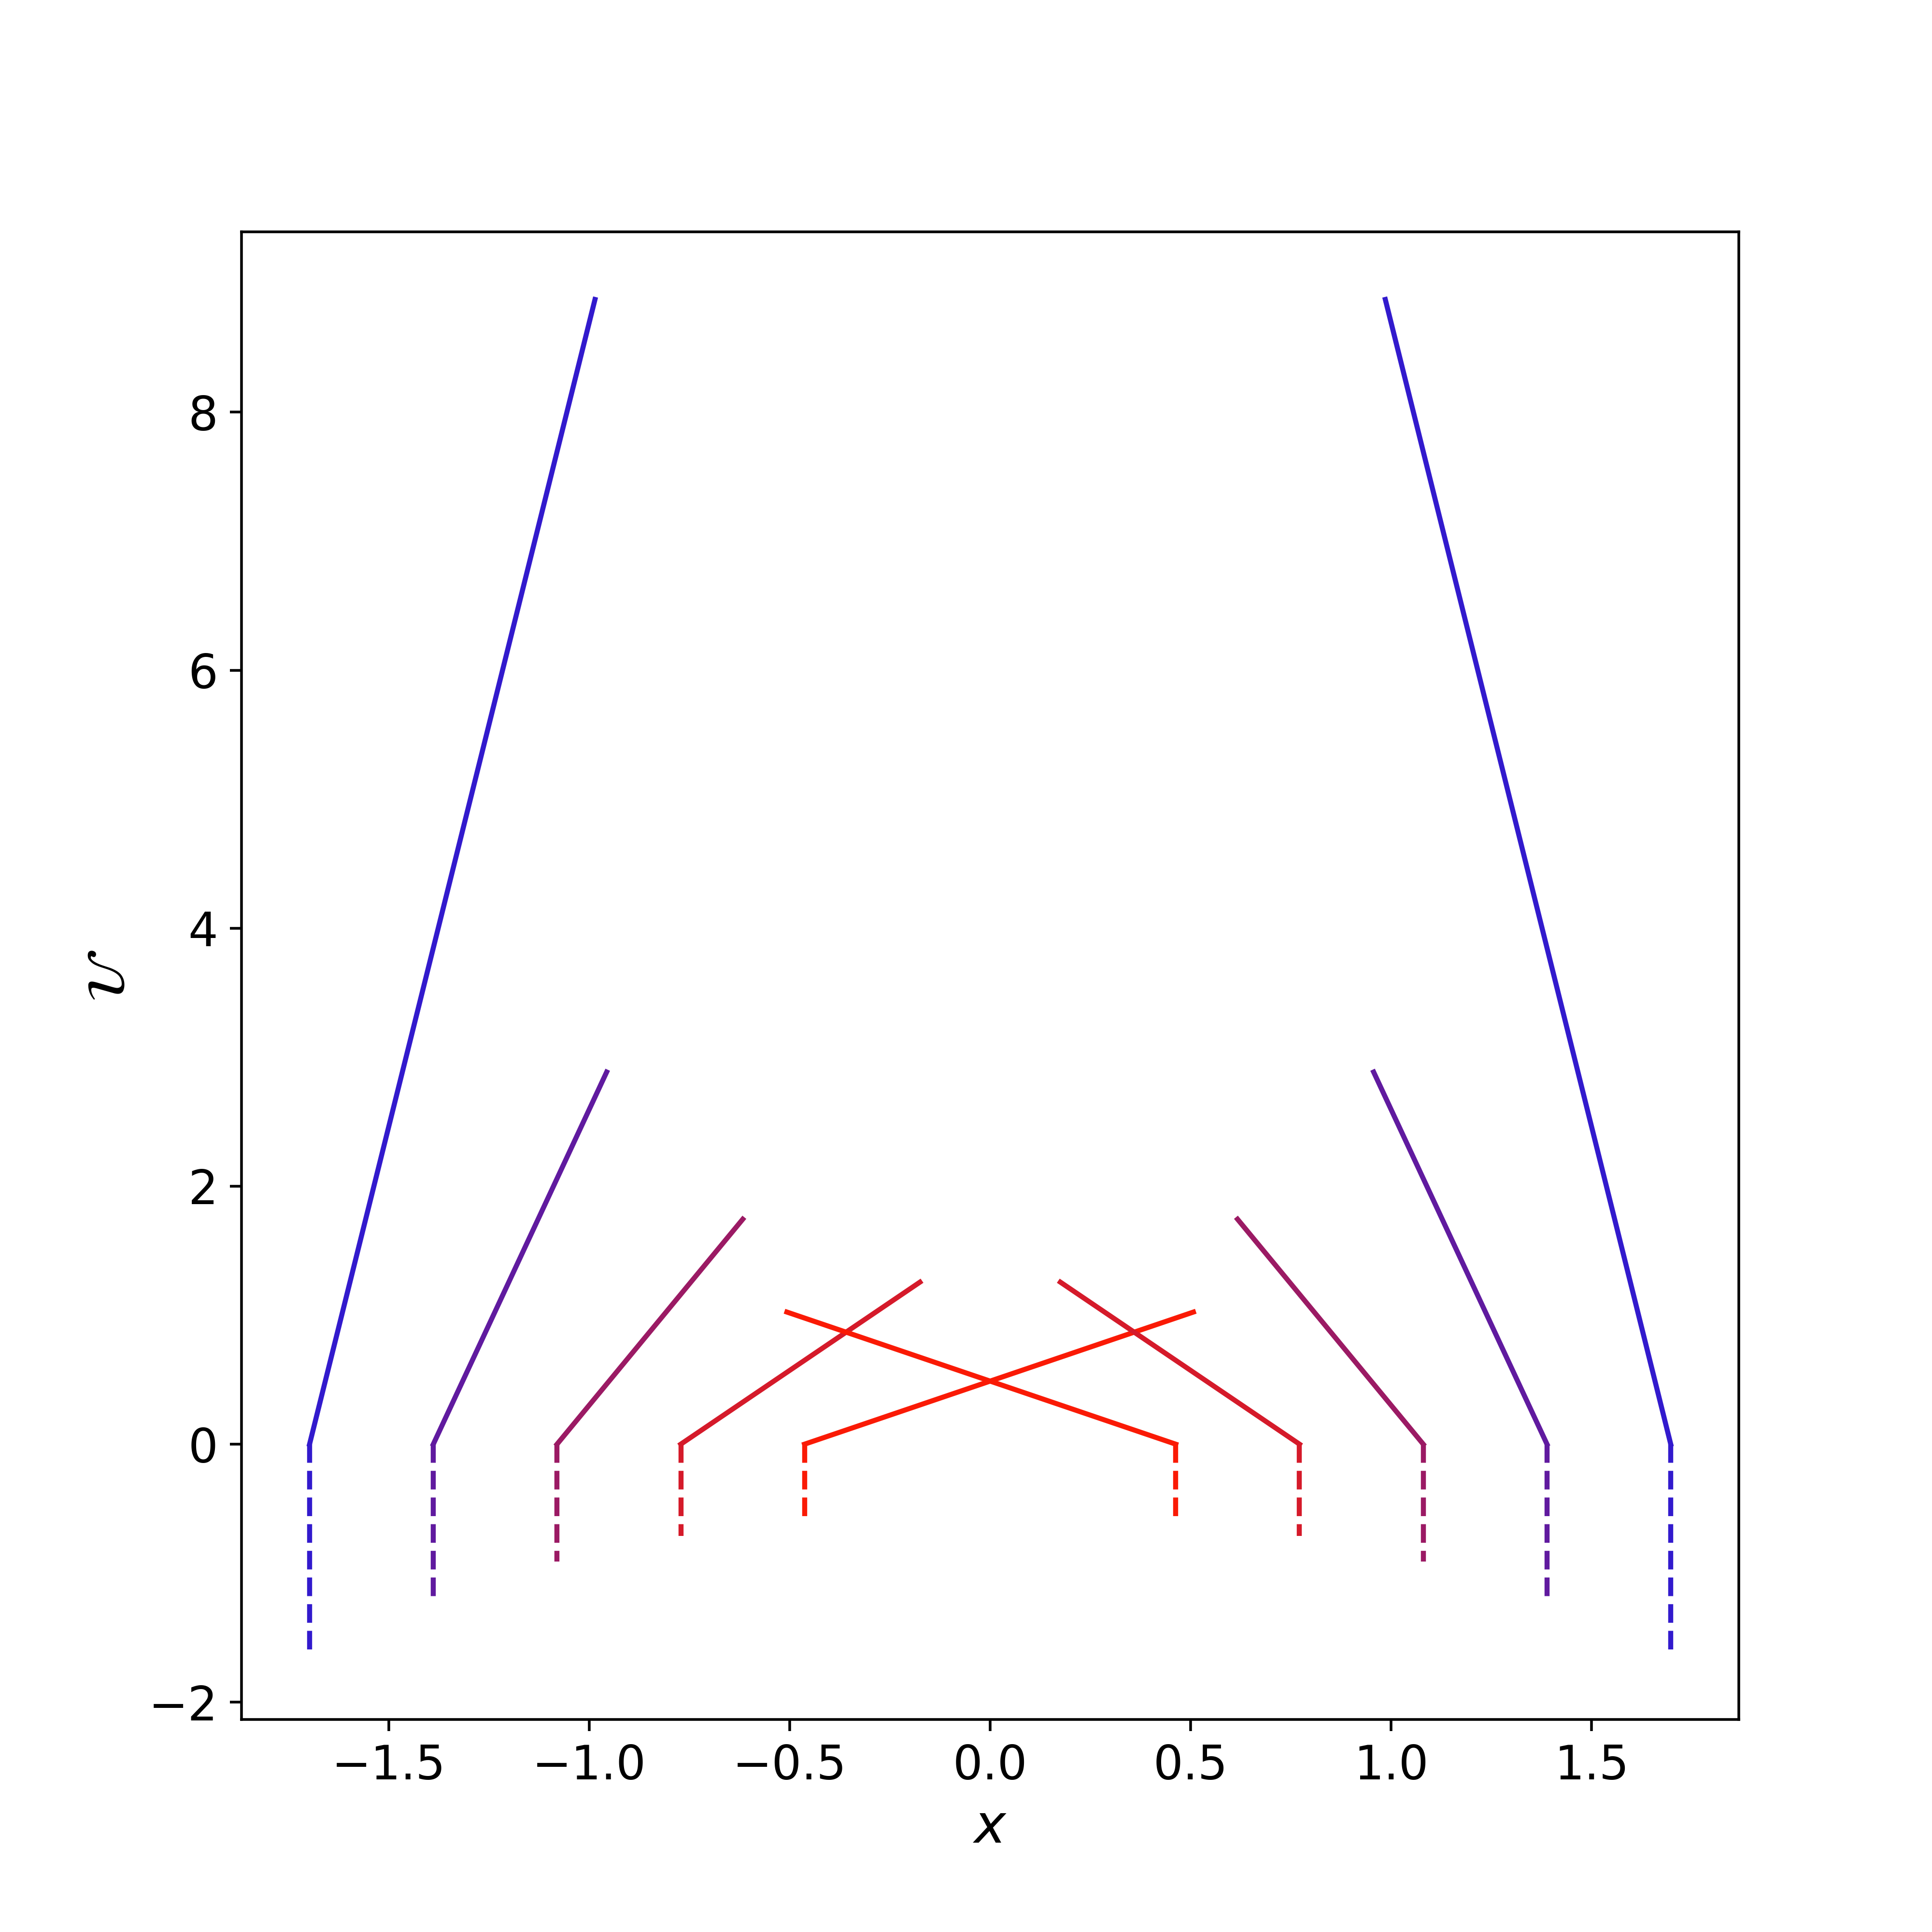
\includegraphics[width=.95\textwidth, clip]{../img/kap02/HT_y-0__xU_mu1_lmb1,5.png}};
            \filldraw[white] (0.29,3.1) circle (4pt);
            \node[text width=7pt] at (0.29,3.1) {\scriptsize{$\matu$}};
            \filldraw[white] (3.25,0.28) circle (4pt);
            \node[text width=7pt] at (3.25,0.28) {\scriptsize{$x$}};
        \end{tikzpicture}
        \caption{$\Lambda = 1,5$}
    \end{subfigure}
    \hfill
    \begin{subfigure}[b]{0.45\textwidth}
        \begin{tikzpicture}
            \node[inner sep=0pt, anchor=south west] (ds) at (0,0)
            {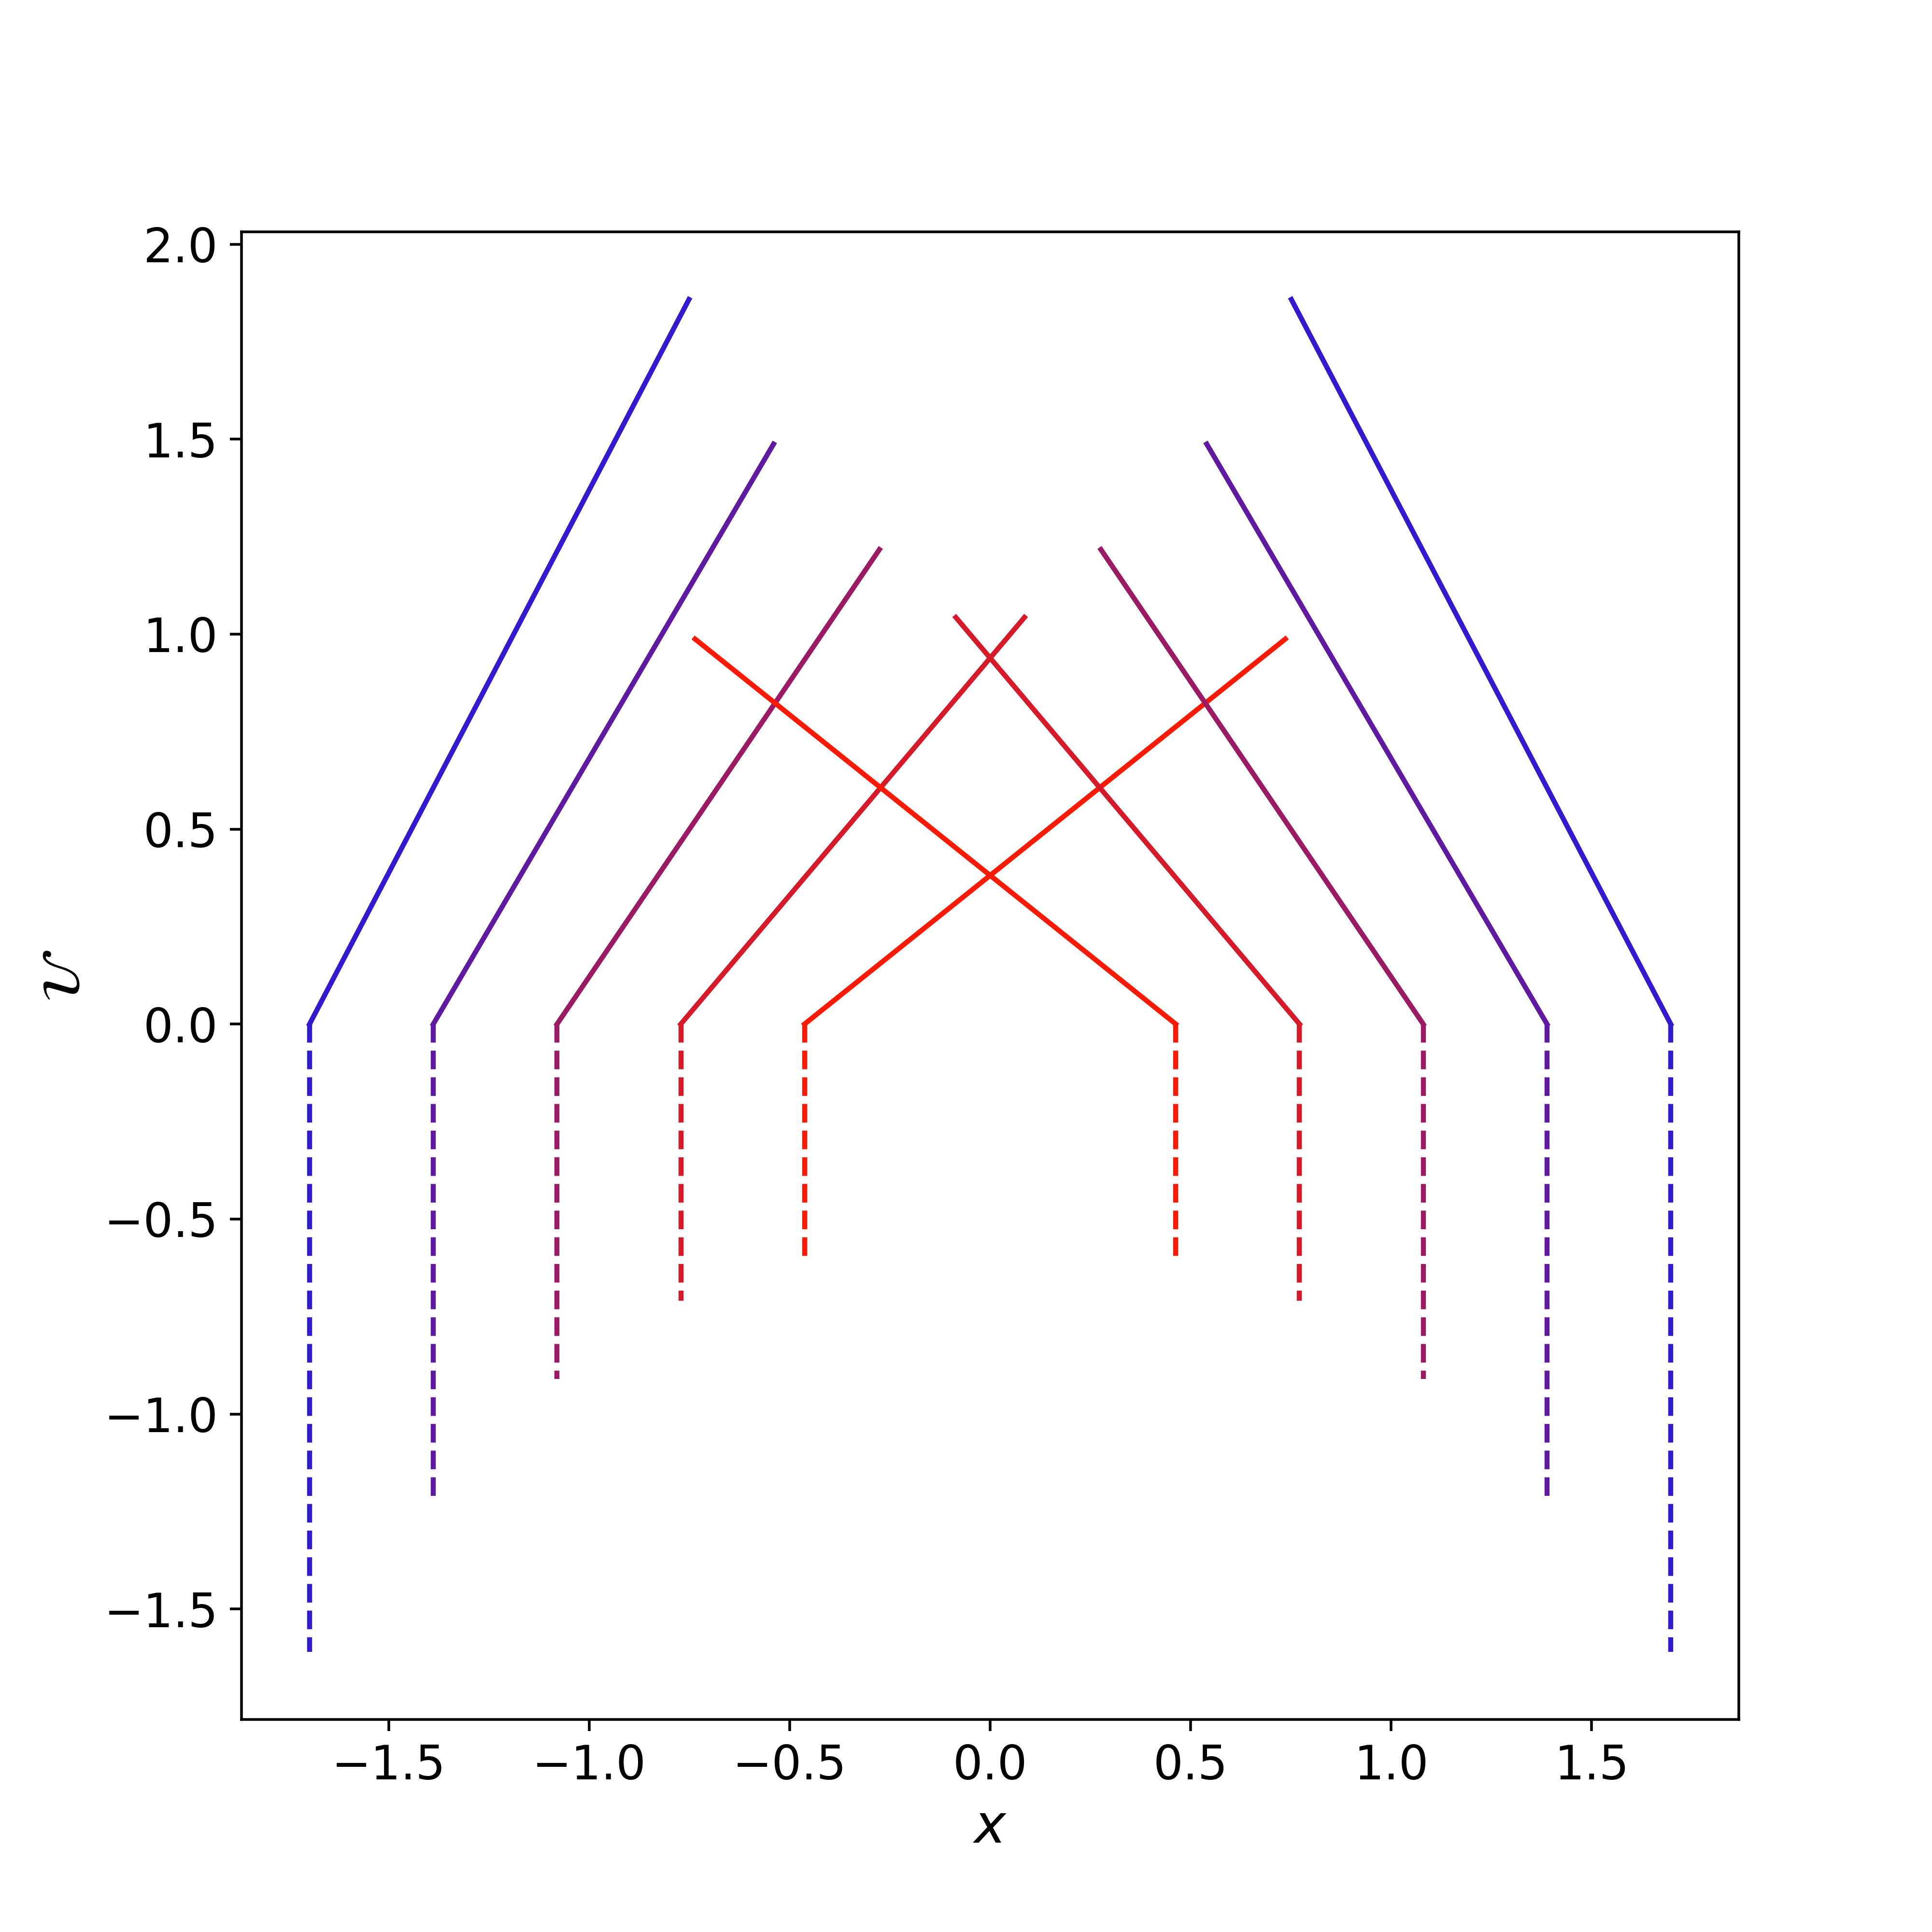
\includegraphics[width=.95\textwidth, clip]{../img/kap02/HT_y-0__xU_mu1_lmb-1,5.png}};
            \filldraw[white] (0.29,3.1) circle (4pt);
            \node[text width=7pt] at (0.29,3.1) {\scriptsize{$\matu$}};
            \filldraw[white] (3.25,0.28) circle (4pt);
            \node[text width=7pt] at (3.25,0.28) {\scriptsize{$x$}};
        \end{tikzpicture}
        \caption{$\Lambda = -1,5$}
    \end{subfigure}
    \caption{Geodetický pohyb nulové částice ($\dot \matu^-=1$, $\dot \matv^-=0$, $\dot \eta^-=0$) v nadploše $y = 0$ v Hottově--Tanakově řešení s parametrem $b_0 = 1$.}
    \label{fig:HottaTanakaNullY0}
\end{figure}

Pro nulové částice nenacházející se na nadploše obsahující osu symetrie dostáváme očekávané strhnutí k
ose symetrie Hottova--Tanakova řešení, k $\eta=0$ (viz obrázek \ref{fig:HottaTanakaNullYsqrt2}). 

\begin{figure}[ht]
    \centering
    \begin{subfigure}[b]{0.45\textwidth}
        \begin{tikzpicture}
            \node[inner sep=0pt, anchor=south west] (ds) at (0,0)
            {\adjincludegraphics[trim={{.08\width} {.1\height} {.12\width} {.15\height}}, width=.95\textwidth, clip]{../img/kap02/HT_y-1__x-y-U_mu1_lmb1.pdf}};
            \filldraw[white] (5,1.2) circle (4pt);
            \node[text width=7pt] at (5, 1.2) {\footnotesize{$\matu$}};
            \filldraw[white] (1.55,1.2) circle (4pt);
            \node[text width=7pt] at (1.55,1.2) {\footnotesize{$x$}};
            \filldraw[white] (0.35,2.85) circle (4pt);
            \node[text width=7pt] at (0.35,2.85) {\footnotesize{$y$}};
        \end{tikzpicture}
        \caption{$\Lambda = 1$}
    \end{subfigure}
    \hfill
    \begin{subfigure}[b]{0.45\textwidth}
        \begin{tikzpicture}
            \node[inner sep=0pt, anchor=south west] (ds) at (0,0)
            {\adjincludegraphics[trim={{.08\width} {.1\height} {.12\width} {.15\height}}, width=.95\textwidth, clip]{../img/kap02/HT_y-1__x-y-U_mu1_lmb-1.pdf}};
            \filldraw[white] (5,1.2) circle (4pt);
            \node[text width=7pt] at (5, 1.2) {\footnotesize{$\matu$}};
            \filldraw[white] (1.55,1.2) circle (4pt);
            \node[text width=7pt] at (1.55,1.2) {\footnotesize{$x$}};
            \filldraw[white] (0.35,2.85) circle (4pt);
            \node[text width=7pt] at (0.35,2.85) {\footnotesize{$y$}};
        \end{tikzpicture}
        \caption{$\Lambda = -1$}
    \end{subfigure}
    \caption{Geodetický pohyb nulových částic ($\dot \matu^-=1$, $\dot \matv^-=0$, $\dot \eta^-=0$) v~nadploše $y = \sqrt{2}$ v Hottově-Tanakově řešení s parametrem $b_0 = 1$.}
    \label{fig:HottaTanakaNullYsqrt2}
\end{figure}

Pro porovnání efektu impulzní vlny na časupodobné testovací částice v konformně plochých souřadnicích byly vykresleny případy geodetického pohybu v prostoročasu bez vlny
a v prostoročasu s impulzní vlnou s parametrem $b_0=3$.

\begin{figure}[ht]
    \centering
    \begin{subfigure}[b]{0.48\textwidth}
        \begin{tikzpicture}
            \node[inner sep=0pt, anchor=south west] (ds) at (0,0)
            {\adjincludegraphics[trim={{.08\width} {.05\height} {.12\width} {.15\height}}, width=.95\textwidth, clip]{../img/kap02/HT1_ring_matter__x-y-U_mu0_lmb1.pdf}};
            \filldraw[white] (0.35,3.46) circle (5pt);
            \node[text width=7pt] at (0.35,3.46) {\footnotesize{$\matu$}};
            \filldraw[white] (5.25,1.05) circle (5pt);
            \node[text width=7pt] at (5.25,1.05) {\footnotesize{$x$}};
            \filldraw[white] (1.75,1.05) circle (5pt);
            \node[text width=7pt] at (1.75,1.05) {\footnotesize{$y$}};
        \end{tikzpicture}
        \caption{de Sitter $(\Lambda = 1)$}
    \end{subfigure}
    \hfill
    \begin{subfigure}[b]{0.48\textwidth}
        \begin{tikzpicture}
            \node[inner sep=0pt, anchor=south west] (ds) at (0,0)
            {\adjincludegraphics[trim={{.08\width} {.05\height} {.12\width} {.15\height}}, width=.95\textwidth, clip]{../img/kap02/HT2_ring_matter__x-y-U_mu3_lmb1.pdf}};
            \filldraw[white] (0.35,3.46) circle (5pt);
            \node[text width=7pt] at (0.35,3.46) {\footnotesize{$\matu$}};
            \filldraw[white] (5.25,1.05) circle (5pt);
            \node[text width=7pt] at (5.25,1.05) {\footnotesize{$x$}};
            \filldraw[white] (1.75,1.05) circle (5pt);
            \node[text width=7pt] at (1.75,1.05) {\footnotesize{$y$}};
        \end{tikzpicture}
        \caption{Hotta--Tanaka$(\Lambda = 1)$}
    \end{subfigure}

    \begin{subfigure}[b]{0.48\textwidth}
        \begin{tikzpicture}
            \node[inner sep=0pt, anchor=south west] (ds) at (0,0)
            {\adjincludegraphics[trim={{.08\width} {.05\height} {.12\width} {.15\height}}, width=.95\textwidth, clip]{../img/kap02/HT3_ring_matter__x-y-U_mu0_lmb-1.pdf}};
            \filldraw[white] (0.35,3.46) circle (5pt);
            \node[text width=7pt] at (0.35,3.46) {\footnotesize{$\matu$}};
            \filldraw[white] (5.25,1.05) circle (5pt);
            \node[text width=7pt] at (5.25,1.05) {\footnotesize{$x$}};
            \filldraw[white] (1.75,1.05) circle (5pt);
            \node[text width=7pt] at (1.75,1.05) {\footnotesize{$y$}};
        \end{tikzpicture}
        \caption{Anti--de Sitter $(\Lambda = -1)$}
    \end{subfigure}
    \hfill
    \begin{subfigure}[b]{0.48\textwidth}
        \begin{tikzpicture}
            \node[inner sep=0pt, anchor=south west] (ds) at (0,0)
            {\adjincludegraphics[trim={{.08\width} {.05\height} {.12\width} {.15\height}}, width=.95\textwidth, clip]{../img/kap02/HT4_ring_matter__x-y-U_mu3_lmb-1.pdf}};
            \filldraw[white] (0.35,3.46) circle (5pt);
            \node[text width=7pt] at (0.35,3.46) {\footnotesize{$\matu$}};
            \filldraw[white] (5.25,1.05) circle (5pt);
            \node[text width=7pt] at (5.25,1.05) {\footnotesize{$x$}};
            \filldraw[white] (1.75,1.05) circle (5pt);
            \node[text width=7pt] at (1.75,1.05) {\footnotesize{$y$}};
        \end{tikzpicture}
        \caption{Hotta-Tanaka $(\Lambda = -1)$}
    \end{subfigure}
    \caption{Časupodobné geodetiky ($\dot \matu^-=\frac{1}{2N}$, $\dot \matv^-=-\frac{1}{N}$, $\dot \eta^-=0$), kde $N$ je normalizační faktor, v (A)--dS a Hottově--Tanakově řešení s parametrem $b_0 = 3$.}
    \label{fig:HottaTanakaMatter}
\end{figure}

Dále vizualizujeme efekt refrakce geodetik v 5--dimenzionálním formalismu. Nulové geodetiky tvoří generátory (A)--dS hyperboloidu, protože při refrakci nedochází
ke změně kauzálního charakteru, po refrakci zůstává geodetika generátorem hyperboloidu, ale, jak vyplývá z refrakčních rovnic \eqref{eq:refraction_velocity_null_cart}, v jiné nadploše - dochází k refrakci
ve všech směrech, kromě směru normály na vlnoplochu. Případ refrakce nulových částic na de Sitterově prostoročasu je na vizualizován na obrázku \ref{fig:HottaTanaka5D}.

\begin{figure}[ht]
    \centering
    \begin{tikzpicture}
        \node[inner sep=0pt, anchor=south west] (ds) at (0,0)
        {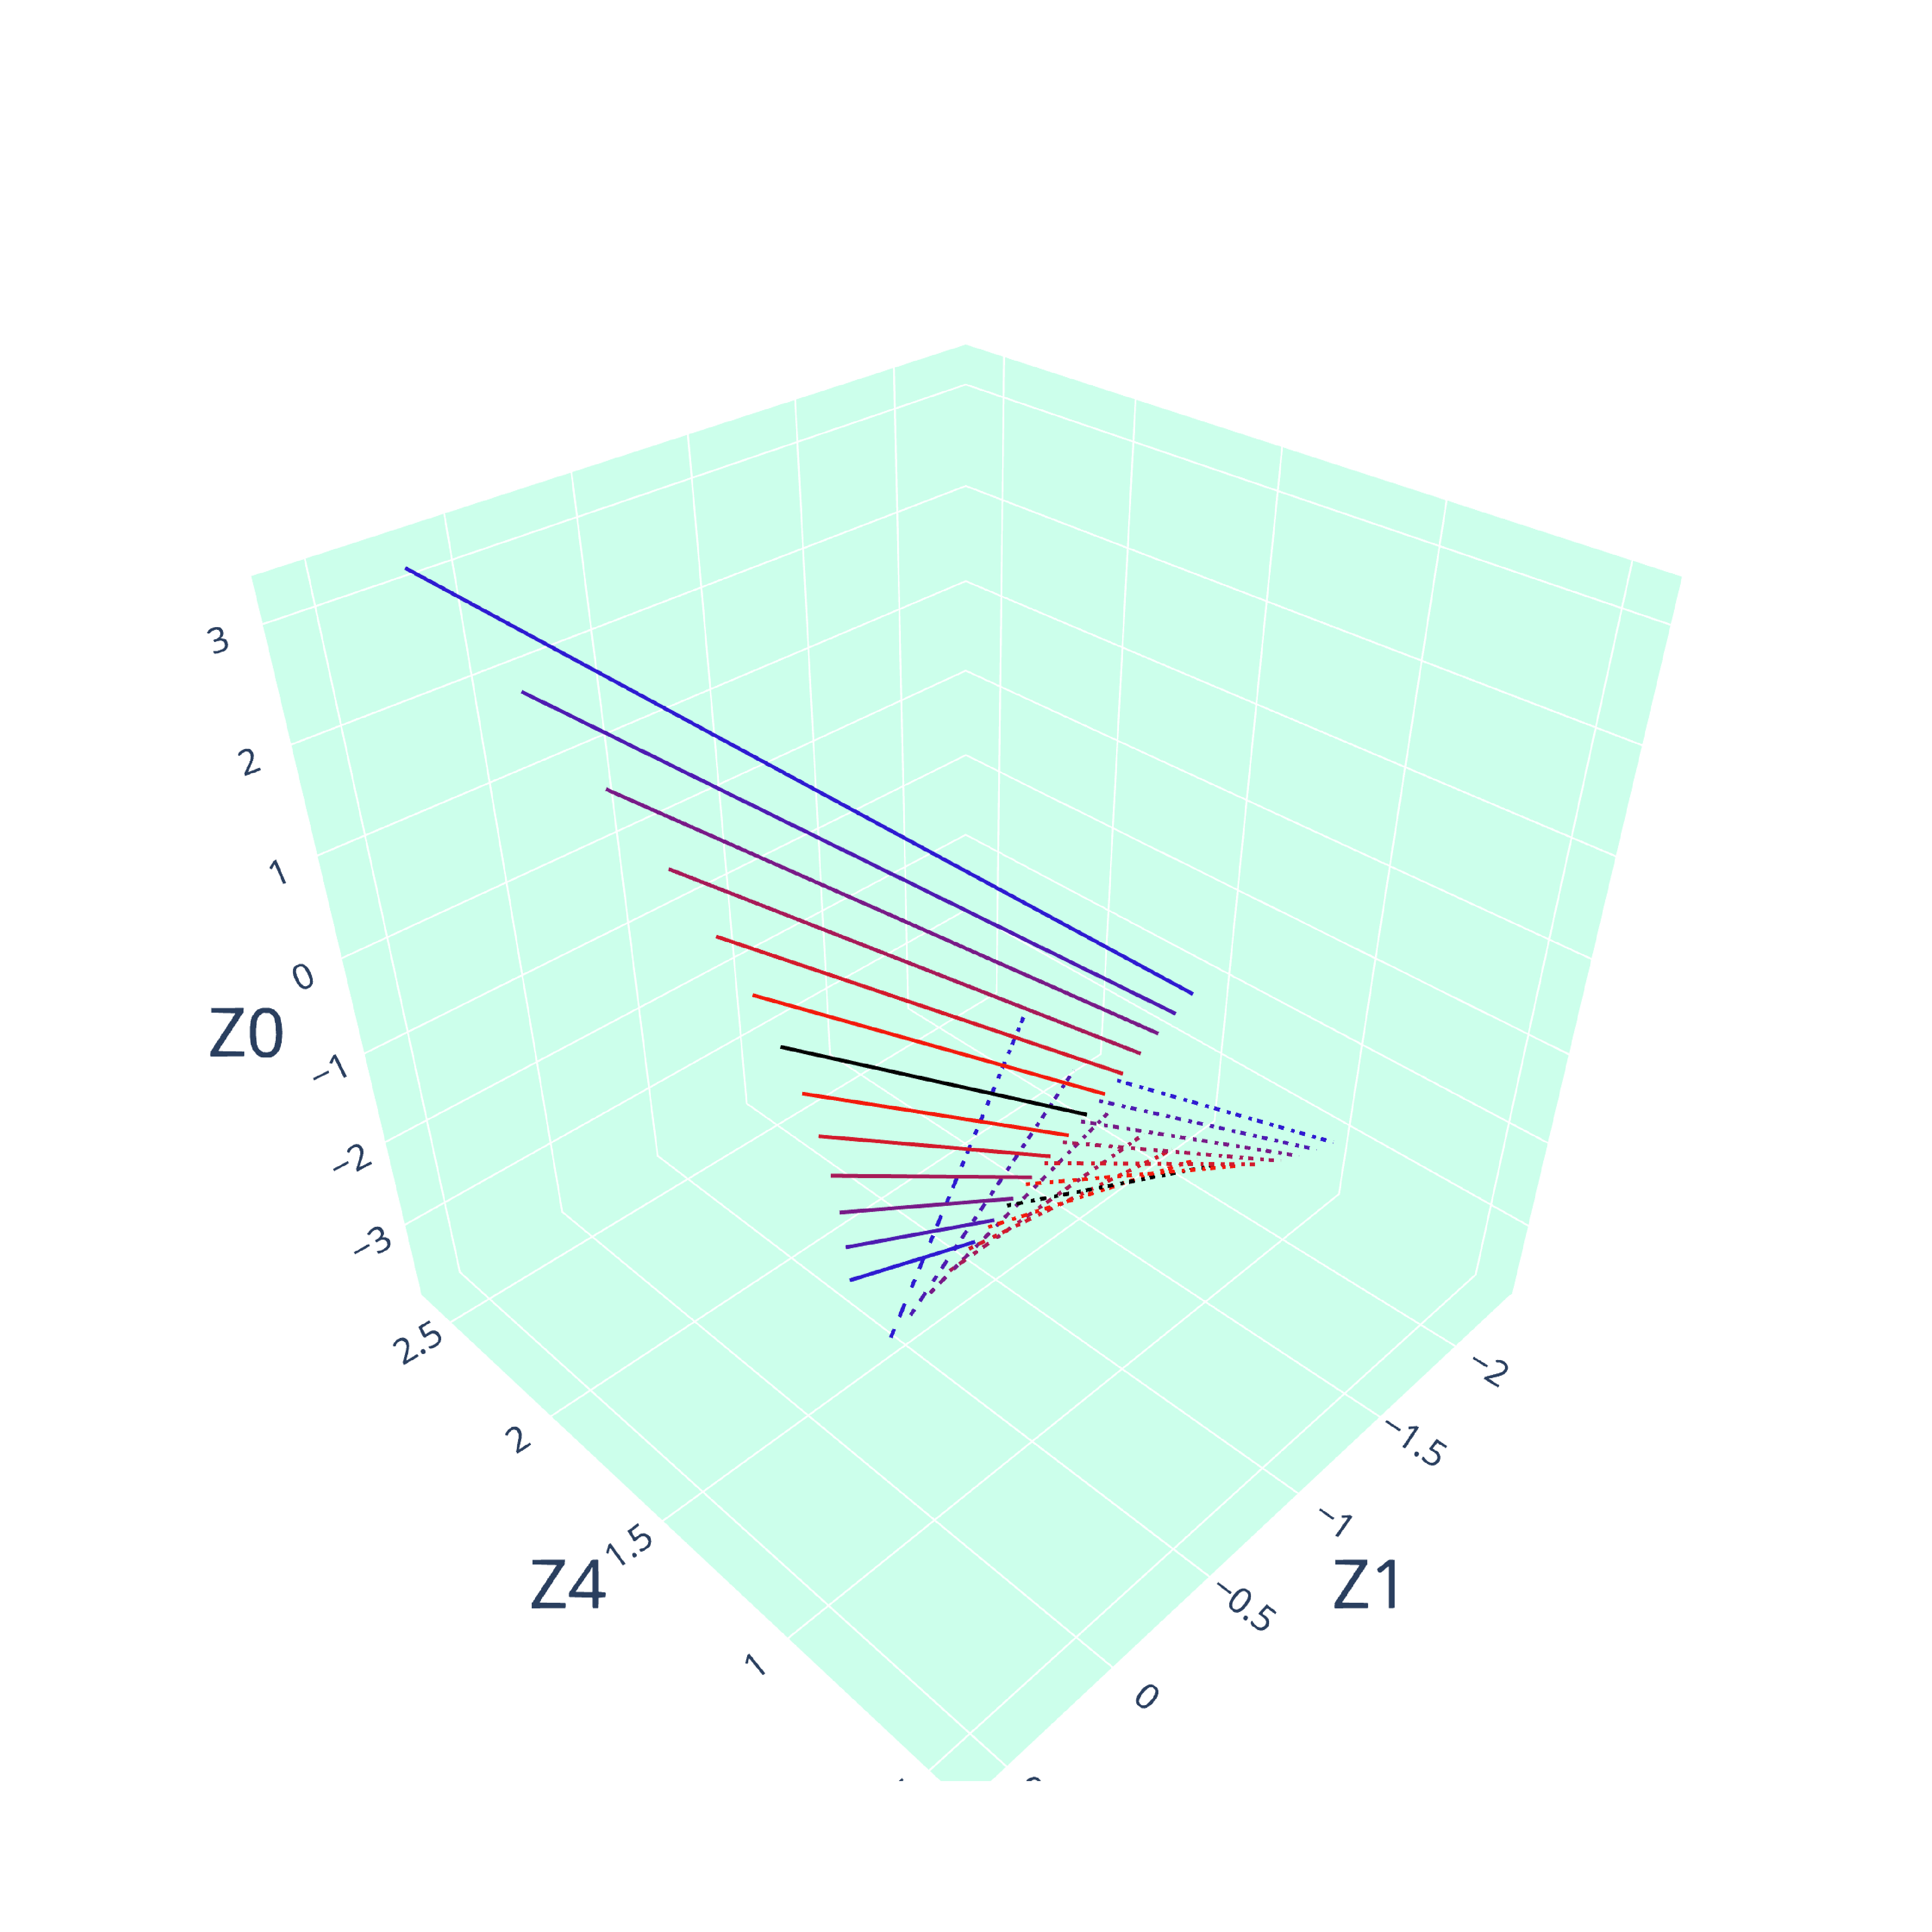
\includegraphics[width=.95\textwidth, clip]{../img/kap02/HT1_x1_null__Z0-Z1-Z4_mu1_lmb1.pdf}};
        \filldraw[white] (1.65,6.35) circle (12pt);
        \node[text width=14pt] at (1.65,6.35) {\normalsize{$Z_0$}};
        \filldraw[white] (4.02,2.33) circle (12pt);
        \node[text width=14pt] at (4.02,2.33) {\normalsize{$Z_4$}};
        \filldraw[white] (9.8,2.4) circle (12pt);
        \node[text width=14pt] at (9.8,2.4) {\normalsize{$Z_1$}};
    \end{tikzpicture}
    \caption{Geodetický pohyb nulové částice ($\dot \matu^-=1$, $\dot \matv^-=0$, $\dot \eta^-=0$) procházející vlnoplochou $\Lambda=1$ Hottova--Tanakova řešení s parametrem $b_0 = 1$ v~$\eta=1,5$ a různých časech (tedy v různých hodnotách souřadnice $\matv$) vyobrazený ve vnoření do $\mathbb{E}^{1,4}$.}
    \label{fig:HottaTanaka5D}
\end{figure}

\cleardoublepage